Este capítulo apresenta os principais conceitos relacionados com a tecnologia blockchain e a forma como cada um deles contribui para a manutenção de suas propriedades. Apesar de existirem diversas variações entre as blockchains, este capítulo tem como foco as plataformas Bitcoin e Ethereum, a primeira por ter sido a pioneira da tecnologia blockchain e a mais conhecida até os dias atuais, e a última por estar diretamente relacionada com este trabalho. Além de expor os aspectos estruturais e funcionais da Ethereum, este capítulo também descreve sobre CIs, vulnerabilidades existentes, e estratégias para mitigação dessas vulnerabilidades, fornecendo um conjunto de conceitos e informações necessárias para o entendimento da proposta deste trabalho.

Na Seção~\ref{tex:fund:blockchain} são introduzidos os fundamentos da tecnologia blockchain. Na Seção~\ref{tex:fund:ethereum} são abordados os conceitos e as particularidades inerentes à blockchain Ethereum. Na Seção~\ref{tex:fund:ethereum:smartc} é discutido sobre o ciclo de execução dos CIs, vulnerabilidades presentes em CIs, e ataques ocorridos que exploraram essas vulnerabilidades. Enfim, algumas estratégias para verificação e detecção de vulnerabilidades são expostas Seção~\ref{tex:fund:verificacao}. 

%---------------------------------------------------------------------%
\section{A tecnologia Blockchain} \label{tex:fund:blockchain}

Com a ascensão das criptomoedas, a DTL tem ganhado visibilidade nos últimos anos. As DTLs são conhecidas também como blockchain, e provêm uma arquitetura descentralizada, que não necessita de confiança em uma entidade central (e.g., o banco central) para gerenciamento das transações, isto é, evita que uma terceira parte acesse as informações dos usuários~\cite{monrat2019survey-blockchain-ieee}. Assim, essa tecnologia, juntamente com a implantação dos CIs, pode potencializar soluções em diversas áreas além da financeira~\cite{swan2015blockchain-book}.

A primeira arquitetura blockchain, apresentada por~\citeonline{overview-bitcoin2008nakamoto}, surgiu com a criptomoeda Bitcoin, que permite aos usuários a realização de transações financeiras de forma pseudo-anônima na internet, sem necessitar de cadastro de uma agência intermediadora. Além da Bitcoin, outras blockchains surgiram nos últimos anos, como a Ethereum, que possibilitou a implantação de CIs, que são programas de computador executados de forma automática, imutável e descentralizada~\cite{ethereum2014whitepaper}. Com os CIs observou-se uma expansão de novas áreas de aplicação das DTLs~\cite{maesa2020blockchain3.0}. Deste modo, esta seção tem como objetivo apresentar os conceitos sobre blockchain Bitcoin e Ethereum, e expor brevemente alguns exemplos de aplicações. Os conceitos descritos a seguir, na Seção~\ref{tex:fund:blockchain:estrutura}, abordam questões gerais sobre a blockchain, e têm como principal referência a Bitcoin. Na Seção~\ref{tex:fund:ethereum} são tratados elementos específicos e exemplos de aplicação da blockchain Ethereum.

\subsection{Estrutura e funcionamento da blockchain} \label{tex:fund:blockchain:estrutura}

Em empresas, utiliza-se um livro-razão para lançamento de registros contábeis para elaboração de relatórios financeiros~\cite{marion1985contabilidade}. Na estrutura de dados de uma blockchain, este livro-razão fica disposto por meio uma cadeia de blocos interligados (i.e., uma lista encadeada) que armazenam todo o histórico de transações, como ilustrado na Figura~\ref{fig:blockchain_estrutura}. Cada participante da rede é responsável por manter uma versão atualizada do histórico de transações e preservar sua integridade~\cite{overview-blockchainbasic2018drescher}. Quando nova transação ocorre, informações como as contas envolvidas, a quantia transferida, a assinatura digital que autorizada a transação, e o horário da transação, são transmitidas entre todos os nós da rede. Os nós da rede, conhecidos como mineradores, coletam uma determinada quantidade de transações e as englobam em um componente chamado de bloco~\cite{overview-blockchainbasic2018drescher}. 

As transações englobadas em um bloco são organizadas na forma de uma árvore de Merkle. Nessa estrutura de dados do tipo árvore cada transação é alocada em um nó folha, e os demais nós armazenam referências do código \textit{hash} gerado a partir dessas transações. Um código \textit{hash} é gerado por meio de algum algoritmo criptográfico de geração de código \textit{hash}, como o SHA-3~\cite{dworkin2015sha3} e o Keccak256~\cite{bertoni2020keccak}. Esses algoritmos recebem e processam dados de entrada, e então geram um código formado por uma sequência de caracteres e dígitos, de forma que, para duas ou mais entradas distintas, a chance de um código \textit{hash} igual ser gerado é extremamente baixa. Outro ponto importante é que, apenas com a posse de um código gerado, não há como se obter os dados de entrada do qual o código se originou.

Na Figura~\ref{fig:blockchain_estrutura} é ilustrada a estrutura da blockchain como um conjunto de blocos interligados em que, a partir dos blocos, as informações das transações podem ser acessadas por meio da raiz da árvore de Merkle. 

\begin{figure}[htb]
 \caption{Estrutura da blockchain}
 \label{fig:blockchain_estrutura}
 \centering
 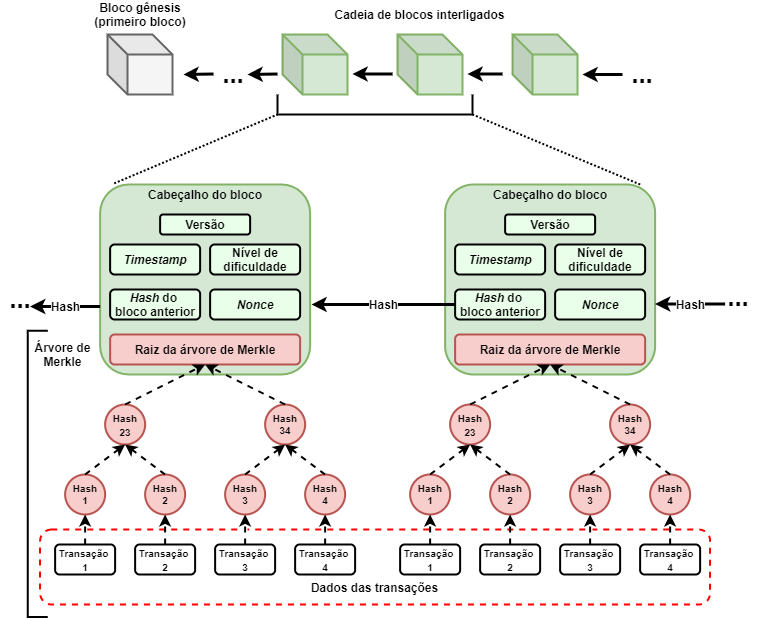
\includegraphics[scale=0.6]{figuras/block_estrutura_cabeçalho.png}
 \fdireta{erikson2020survey-health, overview-dinh-2018}
\end{figure}

Para cada bloco é criado um cabeçalho, que passa a integrar o bloco. As informações presentes no cabeçalho podem variar de acordo com a rede blockchain. Na rede Bitcoin~\cite{overview-bitcoin2008nakamoto}, um cabeçalho é formado por cinco elementos:  
\begin{itemize}
    \item \textbf{Versão:} Número da versão do protocolo de regras de validação a ser seguido; 
    \item \textbf{\textit{Hash} do bloco anterior:} Obtido a partir dos dados do cabeçalho do último bloco presente na blockchain no momento da construção do próximo bloco;
    \item \textbf{Raiz da árvore de Merkle:} Em um bloco, apenas a raiz da árvore de Merkle é armazenada. 
    \item \textbf{\textit{Timestamp}:} Horário atual referente ao momento em que o bloco está sendo criado. Esta informação é essencial para manter a ordenação dos blocos no histórico de transações mantido por cada nó da rede;
    \item \textbf{Nível de dificuldade:} Número que indica o nível de dificuldade do quebra-cabeça computacional que deve ser resolvido pelos mineradores na disputa pela criação do próximo bloco. Este item influencia diretamente no tempo e esforço computacional necessário para a criação de um bloco;
    \item \textbf{\textit{nonce}:} Quando o \textit{nonce} é incorporado ao cabeçalho do bloco, o código \textit{hash} obtido a partir do cabeçalho deve ser iniciado por uma quantidade predefinida de zeros, que é indicada pelo nível de dificuldade. 
\end{itemize}

%%%%%%%%%%% Inserir figura do exemplo do nonce em um bloco

Ao se criar um bloco, o minerador forma primeiro um bloco preliminar contendo os dados dos itens 1 ao 5. Para se obter o \textit{nonce} é necessário realizar uma quantidade massiva de tentativas com o intuito de encontrar a sequência de caracteres e dígitos que satisfaça o nível de dificuldade predefinido. Essa tarefa é conhecidas como mineração, e gera uma disputa entre os nós da rede pela criação do próximo bloco. Nessa disputa, aqueles que possuem computadores mais robustos e com maior capacidade de processamento têm maiores chances de ganhar. A descoberta do \textit{nonce} também é referida neste trabalho como um quebra-cabeça computacional ou quebra-cabeça de \textit{hash}~\cite{overview-blockchainbasic2018drescher, swan2015blockchain-book}. 

%O \textit{nonce} é um item necessário em blockchains nas quais, assim como na \textit{Bitcoin}, utilizam um algoritmo de consenso com regras para criação e validação de blocos conhecido como \textit{proof-of-work}~\cite{overview-bitcoin2008nakamoto}.

Assim que o \textit{nonce} é adicionado ao bloco, este é então transmitido pela rede para que todos os nós possam acessá-lo e participar do processo de validação do bloco. Caso o bloco seja aceito no processo de validação, então cada nó adiciona o bloco válido à própria cópia da estrutura de dados blockchain e o minerador é recompensado pelo esforço empreendido~\cite{overview-bitcoin2008nakamoto}.

%Desta forma, qualquer tentativa de adulterar ou adicionar indevidamente uma transação na árvore referenciada pelo bloco irá invalidar a referência de \textit{hash} da raiz, alterando também o valor do \textit{hash} do bloco;

Como o \textit{hash} gerado nas ramificações da árvore de Merkle depende diretamente do conteúdo das transações, qualquer alteração em uma transação invalida as referências de \textit{hash} dos nós da ramificação da qual a transação pertence, inclusive o nó raiz. Com uma modificação no valor de \textit{hash} da árvore de Merkle, o valor de \textit{hash} do bloco também é alterado. Assim, alterar o valor de \textit{hash} do bloco invalida a referência de \textit{hash} que aponta para o cabeçalho do bloco modificado, invalidando, assim, toda a estrutura de dados~\cite{antonopoulos2014mastering}.

Desta forma, tentar fraudar dados de transação manipulados envolve uma série de operações custosas. Primeiro deve-se reescrever a árvore de Merkle à qual a transação manipulada pertence. Após isso, é necessário reescrever o cabeçalho do bloco a qual a raiz da árvore de Merkle reescrita pertence, o que requer a solução do quebra-cabeça de \textit{hash} para obtenção de um novo \textit{nonce}. Consequentemente, todos os cabeçalhos até o final da estrutura de dados da blockchain precisam ser reescritos, o que inclui encontrar o \textit{nonce} de cada um. Este processo é propositalmente complexo e se faz necessário para manter os dados consistentes e íntegros. Isso atribui à tecnologia blockchain a propriedade de imutabilidade~\cite{antonopoulos2014mastering, overview-blockchainbasic2018drescher}.

%Elaborar a figura da construção do bloco baseado na imagem de \cite{consenso-Bouraga2021}

%---------------------------------------------------------------%
\subsection{Processo de validação na blockchain} \label{tex:fund:blockchain:consenso}

Um fator fundamental no êxito da Blockchain foi sua capacidade de garantir integridade e confiança em um ambiente de sistemas P2P puramente distribuídos, onde há um número ilimitado de nós conectados sem nenhum nível de confiança pré-estabelecidos entre estes~\cite{overview-blockchainbasic2018drescher}. Em uma rede de blocos com informações que podem ser produzidas por qualquer nó conectado, há o risco iminente de inserção de informações falsas e maliciosas. Para garantir a confiança de que os blocos na blockchain são legítimos, é necessário verificar a validade de um novo bloco antes deste ser inserido na rede. Para incentivar os nós a manterem a integridade das transações, são definidos mecanismos de incentivo, assim como formas de punição para os nós que tentam inserir ou validar transações maliciosas. Em uma blockchain, as regras que regem esse protocolo são definidas por um algoritmo de consenso~\cite{overview-consenso2017sankar, consenso-zhang2020analysis, consenso-Bouraga2021}.

%Por meio de um protocolo previamente estabelecido, os nós são responsáveis por chegar a um consenso para validar cada inserção, seguindo a ordem na qual as transações ocorrem. 

Neste trabalho, o termo ``protocolo de consenso'' é usado para se referir de forma generalizada ao processo de tomada de decisão coletiva entre os nós para validação de novos blocos, um procedimento pertinente em qualquer rede blockchain. Contudo, em cada rede blockchain, esse protocolo pode ser composto por regras distintas. Cada conjunto específico de regras para estabelecimento de um protocolo de consenso é referido neste trabalho como um algoritmo de consenso, que pode apresentar diversas variações.

Um algoritmo de consenso é elaborado com o objetivo de garantir que todos os nós da rede concordem com o histórico da transações que compõem os blocos da rede, que será comum a todos, formando assim a rede blockchain~\cite{consenso-xiao-2020}. Desta forma, os nós são estimulados a participar do processo de validação. Além de proporcionar um ambiente participativo para criação e validação dos blocos, os algoritmos de consenso propõe formas de recompensar os nós honestos, isto é, aqueles que trabalham para manter a integridade da rede e não agem de forma maliciosa~\cite{overview-consenso2017sankar}. 

Cada blockchain pode utilizar uma variação de diferentes algoritmos de consenso. Dentre os principais algoritmos de consenso estão o \sigla{PoW}{\textit{Proof-of-Work}}, \sigla{PoS}{\textit{Proof-of-Stake}} e \sigla{PBFT}{\textit{Practical Byzantine Fault Tolerance}}. Os próximos parágrafos descrevem os fundamentos desses protocolos de consenso.

O protocolo \textbf{PoW} tem entre seus principais mecanismos a competição entre os mineradores para resolução de um quebra-cabeça criptográfico para definir ou \textit{nounce} do bloco. O nó que encontrar o \textit{nounce} primeiro obtém o direito de validar o bloco, que é então criado, dissipado pela rede de nós para que todos os participantes possam verificar sua validade, e, por fim, adicionado à blockchain. O esforço computacional exigido para obtenção do \textit{nounce} tem como consequência um alto consumo de energia. Para estimular a participação honesta dos nós no processo de mineração e compensar os custos financeiros envolvidos neste processo, algoritmos de PoW utilizados em blockchains como Bitcoin e Ethereum oferecem uma recompensa ao vencedor. Esta recompensa é feita por meio da obtenção da posse, por parte do minerador, de uma quantidade da moeda virtual utilizada como incentivo na rede, que pode posteriormente ser convertida em valor monetário (i.e., alguma moeda fiduciária)~\cite{overview-bitcoin2008nakamoto, ethereum2014whitepaper, overview-blockchainbasic2018drescher}. O alto esforço computacional e gasto energético despendido pelos mineradores agrega integridade aos blocos, pois não é vantajoso para um nó malicioso ter um alto gasto para resolução do \textit{nouce} de um bloco com transações fraudadas e correr o risco iminente do bloco ser rejeitado no processo de validação. Por outro lado, um gasto computacional muito elevado pode restringir as condições de acesso dos usuários ao processo de mineração, além de aumentar o tempo para inclusão das transações, limitando questões práticas de implantação e uso de sistemas, como escalabilidade e performance~\cite{consenso-Bouraga2021}.

O algoritmo \textbf{PoS} foi proposto inicialmente por \citeonline{overview-pos-king2012ppcoin} com o intuito de mitigar a dependência do alto consumo de energia e recursos computacionais do PoW~\cite{overview-bitcoin-energy2014}. No PoS, os nós que se candidatam para participar da criação dos blocos, chamados de validadores, investem uma quantia da criptomoeda vigente na blockchain. Esta quantia também é referida como valor de participação, e funciona como uma conta bloqueada com um saldo que representa o comprometimento do validador em manter a integridade da rede. Quanto maior o valor, maior a chance do validador ser selecionado para criar o próximo bloco. Enquanto no PoW a chance do minerador criar um bloco é proporcional ao seu poder computacional, no PoS a chance é proporcional ao valor de participação investido pelo validador~\cite{consenso-xiao-2020, overview-dinh-2018}.

Baseado no trabalho de \citeonline{overview-byzantine1999castro}, o \textbf{PBFT} é adotado na blockchain por meio de dois tipos de nós, o cliente e o servidor. O nó cliente envia um bloco aos nós servidores, e se o bloco for validado por um número suficiente de nós, então este é adicionado à blockchain. Este processo de validação das transações do PBFT consiste em cinco etapas: (i) o nó cliente envia o bloco proposto para os servidores; (ii) os servidores transmitem o bloco para outros servidores, que devem avaliar uma série de condições relacionadas à validade do bloco e chegar a um consenso sobre sua aceitação; (iii) Se o bloco for aceito, o segundo grupo de servidores enviam uma mensagem aos outros nós indicando que o bloco está pronto. Assim que esta mensagem é verificada e validada por um número suficiente de nós, estes entram em fase de ``entrega''; (iv) após realizar a confirmação, cada nó transmite uma mensagem para a rede para atestar sua ação; e (v) o nó servidor que enviou o bloco recebe a resposta, seja o bloco validado ou não~\cite{consenso-Bouraga2021,consenso-xiao-2020,overview-ahmed-2019,consenso-zhang2020analysis}. 

%Apesar de ser crucial para o sucesso de blockchains como Bitcoin e Ethereum, o algoritmo PoW impõe limitações de escalabilidade, performance e participação na rede. Essas questões motivaram pesquisadores e empresas a desenvolver alternativas para mitigação desses problemas, como os algoritmos PoS e PBFT. 

Em dezembro de 2020 foi iniciada a primeira fase de implantação da \textit{Ethereum} 2.0~\footnote{\url{https://github.com/ethereum/eth2.0-specs}}, uma nova rede blockchain que utiliza o algoritmo de consenso PoS. Com isso, pretende-se aumentar a velocidade de validação das transações e integração dos blocos, expandindo a escalabilidade e otimizando a performance das aplicações.

O algoritmo PBFT é utilizado pela \textit{Hyperledger Fabric}~\footnote{\url{https://www.hyperledger.org/use/fabric}}, uma plataforma blockchain privada desenvolvida pela Fundação Linux~\cite{overview-hyperledger2018androulaki}. Assim como o PoS, o PBFT também proporciona economia de energia para validação e integração das transações. Variações do PBFT também são empregadas nas blockchains Stellar~\cite{overview-stellar2015mazieres} e Ripple~\cite{overview-schwartz2014ripple}~\cite{overview-ahmed-2019, consenso-xiao-2020, consenso-zhang2020analysis}.
 
%------- Parágrafo descartado ---------
%Os protocolos de consenso desempenham um papel crucial para o sucesso das tecnologias baseadas em blockchain. A rede Bitcoin, especificada por \citeonline{overview-bitcoin2008nakamoto}, aliou diversos conceitos para descrição do algoritmo de consenso PoW, o que fez do Bitcoin o foi o primeiro caso de sucesso de uma tecnologia capaz de fornecer integridade e segurança em um sistema ponto a ponto puramente distribuído para gerenciamento de posses (i.e., da criptomoeda Bitcoin). Porém, problemas relacionados com o alto gasto em \textit{hardware} e energia para criação dos blocos, e com a espera significativa para integração dos blocos na rede (em torno de 10 minutos na Bitcoin).

\subsection{Escolha do histórico de transações}

O funcionamento da blockchain exige um ritmo de trabalho dos mineradores no qual, em algum momento, estes sempre estarão concentrados em alguma das seguintes tarefas: analisar um novo bloco criado por algum nó da rede; ou se esforçar para criar o próximo bloco que, posteriormente, será analisado pelos demais nós~\cite{overview-blockchainbasic2018drescher}.

A capacidade de transmissão e entrega de novos blocos sofre grande influência da capacidade da entrega de mensagens de rede. Por consequência, vários nós podem terminar de construir um bloco em um pequeno intervalo de tempo. Esses blocos são transmitidos pela rede e coletados pelos nós em momentos distintos. Assim, os nós da rede não terão informações idênticas à sua disposição ao mesmo tempo~\cite{overview-blockchainbasic2018drescher}. 

Quando um nó coleta em sua caixa de entrada mais de um bloco com o mesmo valor de referência do \textit{hash} do bloco anterior, então uma ramificação, referida também como um \textit{fork}, é criada, já que esses blocos possuem o mesmo bloco pai. Essas ramificações podem formar uma cadeia com diversos blocos. Dessa forma, a estrutura de dados da blockchain pode ser vista como uma árvore, porém, quando ocorre um \textit{fork}, os nós da rede devem escolher apenas uma ramificação para compor a cadeia de blocos principal. Na Bitcoin é definido que, sempre que ocorrer um \textit{fork}, deve-se escolher a cadeia mais longa, ou, em caso de empate, mantém-se aquela que foi recebida primeiro.~\cite{overview-blockchainbasic2018drescher, sompolinsky2015ghost-original}.

%Assim, a ramificação com mais blocos interligados é escolhida. Como o algoritmo PoW exige uma disputa entre os mineradores que envolve poder computacional para a criação de um bloco, então a ramificação com mais blocos é também aquela com o maior esforço computacional dispendido~\cite{overview-bitcoin2008nakamoto}.  

Em situações de decisão como essa, o protocolo da Bitcoin estabelece que a ramificação escolhida pela maioria dos nós é considerada como parte da cadeia de blocos principal, como ilustrado na Figura~\ref{fig:cadeia_blocos}. Este procedimento é estabelecido pelo protocolo de consenso da blockchain e visa manter a integridade da blockchain por meio do consenso alcançado entre os nós participantes. Porém, deve-se considerar a premissa de que sempre haverá mais de 50\% de participantes dispostos a agir de forma honesta~\cite{overview-bitcoin2008nakamoto}. 

\begin{figure}[htb]
 \caption{Cadeia de blocos de uma blockchain}
 \label{fig:cadeia_blocos}
 \centering
 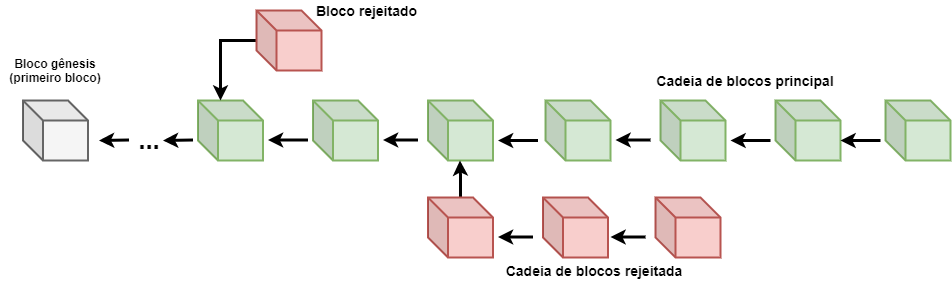
\includegraphics[scale=0.4]{figuras/cadeia_de_blocos.png}
 \fdireta{monrat2019survey-blockchain-ieee}
\end{figure}
 
%-------------------------------------------------------------%
\subsection{Criptografia e autorização de transações} \label{tex:fund:blockchain:cripto}

Para manter a segurança e integridade das transações, é essencial que apenas o proprietário legítimo de uma conta possa transferir o direito de propriedade ou de posse associado à sua conta (e.g., uma quantia de criptomoeda) para outra conta. Com o objetivo de garantir que somente o proprietário legítimo transfira a posse, é utilizada uma assinatura digital. Para isso, é aplicada a criptografia de curva elíptica~\cite{koblitz1987elliptic-curve}, na qual são utilizadas técnicas de \textit{hash} e criptografia assimétrica por meio do par de chaves que cada nó detém, uma chave pública e outra privada. A chave privada fica disponível apenas para seu proprietário, e é utilizada para criptografar informações, transformando-as em um texto cifrado. Por se tratar de uma criptografia assimétrica, não há como se obter a informação original a partir do texto cifrado resultante. A única forma de descriptografar esse texto e obter novamente a informação original é utilizando a chave pública correspondente, que é única para cada proprietário e representa o identificador de sua conta. A chave pública é compartilhada com todos, assim, qualquer nó pode usá-la para se certificar de que a transação foi autorizada por quem cedeu a posse~\cite{overview-blockchainbasic2018drescher, overview-ahmed-2019}.

A assinatura é utilizada em duas situações: (i) na assinatura de uma transação; (ii) e na verificação de uma transação~\cite{overview-ahmed-2019}. Na Figura~\ref{fig:retemente-assinatura-digital} é ilustrado um exemplo em que o proprietário da conta que cede a posse realiza a assinatura da transação por meio dos passos a seguir:
\begin{enumerate}
    \item Descreve a transação com todas a informações necessárias, exceto a assinatura;
    \item Gera o valor de \textit{hash} dos dados de transação;
    \item Utiliza sua chave privada para gerar o valor de \textit{hash} da transação a partir do valor gerado no passo 2. Esse processo é chamado de encriptação;
    \item Adiciona o texto cifrado criado no item 3 à transação como sua assinatura digital.
\end{enumerate}

\begin{figure}[htb]
 \caption{Processo de assinatura digital de uma transação}
 \label{fig:retemente-assinatura-digital}
 \centering
 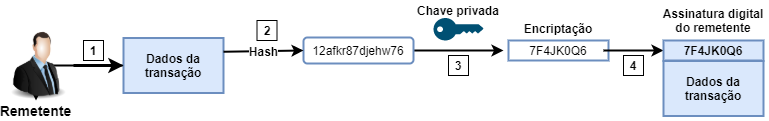
\includegraphics[scale=0.6]{figuras/remetente_assinatura_digital.png}
 \fdireta{overview-ahmed-2019}
\end{figure}

O processo de verificação de uma transação é ilustrado na Figura~\ref{fig:verifica-assinatura-digital}, no qual o nó verificador executa os seguintes passos:
\begin{enumerate}
    \item Cria o valor de \textit{hash} a partir dos dados da transação a ser verificada, com exceção da assinatura;
    \item Utiliza a chave pública da conta que está cedendo a posse para descriptografar a assinatura digital da transação. Esse processo é chamado de decriptação;
    \item Compara o valor do \textit{hash} gerado no passo 1 com o valor obtido no passo 2. Se ambos forem idênticos, então indica que a transação foi autorizada pelo proprietário da chave privada, que corresponde à chave pública que está cedendo a posse (i.e., o identificador da conta). Caso os valores não sejam idênticos, então conclui-se que o proprietário da chave privada não autorizou a transação, que é descartada. 
\end{enumerate}

\begin{figure}[htb]
 \caption{Processo de verificação da assinatura digital de uma transação}
 \label{fig:verifica-assinatura-digital}
 \centering
 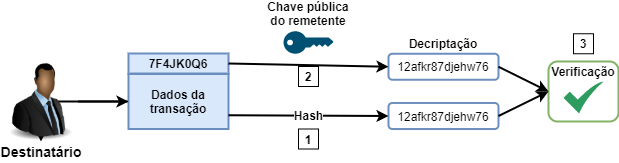
\includegraphics[scale=0.5]{figuras/verifica_assinatura_digital.png}
 \fdireta{overview-ahmed-2019}
\end{figure}

Um valor de \textit{hash} criptográfico é único para cada transação. Analogamente, a associação entre uma chave pública e uma privada também é único. Essa característica faz com que as assinaturas digitais sejam apropriadas para servir como prova de que o proprietário da chave privada usada para criar a assinatura digital realmente concorda com o conteúdo da transação~\cite{overview-blockchainbasic2018drescher}.

%-----------------------------------------------------------------%
\section{Blockchain Ethereum} \label{tex:fund:ethereum}

%No trabalho de \cite{wang2019detecting-nondeterministic-26} a execução de CIs e das transações é vista analisada sob a perspectiva de não-determinismo, isto é, a execução de uma transação possui comportamento não determinístico. Além disso, também é fornecido um overview bem direto e sucinto sobre transações na Ethereum, CIs e MVE. Também, algumas vulnerabilidades conhecidas, como reentrância e \textit{transfer order dependency} são revisadas e exemplificadas do ponto de vista de problemas do não-determinismo.

A Ethereum~\cite{ethereum2014whitepaper} é uma das mais conhecidas implementações da tecnologia blockchain. Ela é definida como uma plataforma de computação distribuída composta por uma rede de computadores que operam de forma descentralizada, autônoma e democrática~\cite{wood2014ethereum-yellow-paper}. Embora também lide com geração e gerenciamento de posse de sua criptomoeda, o Ether, essa é apenas uma parte do que a plataforma é capaz de prover.

O funcionamento da Ethereum baseia-se na implantação de CIs, que são programas de computador que, uma vez implantados, executam automatica e obrigatoriamente  de acordo a lógica definida em sua programação. Por meio desses programas é possível estabelecer um acordo entre duas ou mais partes envolvidas, que se comprometem a cumprir as regras estabelecidas expressas em código. Quanto compilado, um CI é convertido em um \textit{bytecode}, uma representação de baixo nível utilizada para sua execução. Os contratos são executados de forma descentralizada por todos os participantes da rede por meio da \sigla{MVE}{Máquina Virtual Ethereum}~\cite{overview-chen2020blockchain-graph}.

Na Ethereum, as transações são disparadas por meio de mensagens, que podem conter instruções que causam a alteração na estado da blockchain~\cite{wood2014ethereum-yellow-paper}. Isso acontece, por exemplo, quando um nó executa uma função de um CI que altera o valor de algum atributo. Essas transações são coletadas pelos nós para formação dos blocos e são estruturadas em uma \textit{trie}, que é uma variação da árvore de Merkle feita especialmente para uso na Ethereum, e opera de forma semelhante na garantia da imutabilidade dos dados~\cite{wood2014ethereum-yellow-paper}.

A Ethereum foi elaborada por~\citeonline{ethereum2014whitepaper} para ser um protocolo alternativo para criação de DApps. Na plataforma \textit{State of The DApps}~\footnote{\url{https://www.stateofthedapps.com/}} há mais de 3800 DApps contabilizados, sendo que destes, pouco mais de 3 mil utilizam a Ethereum. Nas DApps, geralmente o \textit{front-end} é implementado como uma aplicação \textit{web}, enquanto que o \textit{back-end} é implementado por um ou mais CIs~\cite{survey-Hewa2021smart-contract}. Os números envolvendo a plataforma ajudam a dimensionar o tamanho de sua popularidade. Em 2021 o valor de mercado da Ethereum superou 400 bilhões de dólares, sendo a segunda maior plataforma blockchain em valor de mercado, atrás apenas da Bitcoin, com cerca de 900 bilhões~\footnote{Dados obtidos da CoinMarketCap, disponíveis em: \url{https://coinmarketcap.com/}.}. Além disso, de acordo com a plataforma Etherscan~\footnote{\url{https://etherscan.io/}}, há ao menos 2 milhões de CIs já executados.
% talvez deva colocar essas informações na introdução

Devido às tecnologias e técnicas que compõe a Ethereum, as aplicações que a utilizam dispõe de uma série de propriedades~\cite{ethereum2014whitepaper, survey-Hewa2021smart-contract}, tais como:
%revisar
\begin{itemize}
    \item \textbf{Descentralização}: Eliminação da necessidade de confiança em uma terceira parte reguladora para execução da lógica do contrato;
    \item \textbf{Imutabilidade}: Uma vez executado, o código não pode ser alterado, assim como as transações resultantes da interação entre os contratos e os nós;
    \item \textbf{Persistência dos dados}: Uma vez inseridas na blockchain, as informações contidas em um bloco estarão sempre disponíveis;
    \item \textbf{Execução autônoma}: A execução de condições programadas e fluxo de eventos a serem realizados são disparados automaticamente conforme o sistema blockchain atinge um determinado estado, garantindo a autonomia da execução. O estado no qual uma ação é disparada é definido na programação do CI, em comum acordo com todas as partes envolvidas;
    \item \textbf{Acurácia}: Assim que o CI é executado, confia-se que as condições programadas serão cumpridas. A acurácia da execução do que foi programado é garantida por meio da transparência envolvida na execução autônoma, pois assim, vieses humanos e erros que podem acontecer em uma execução centralizada são evitados.
\end{itemize}

A seguir, na Seção~\ref{tex:fund:ethereum:clientes}, são abordados os tipos de contas que operam na plataforma Ethereum. Detalhes sobre as transações e troca de mensagens  são tratados na Seção~\ref{tex:fund:ethereum:transacao-msgs}. Detalhes sobre a formação dos blocos e seu processo de validação são discutidos nas Seções~\ref{tex:fund:ethereum:blocos} e ~\ref{tex:fund:ethereum:valida}, respectivamente. Alguns exemplos de aplicações baseadas em CIs que executam sobre a plataforma Ethereum são expostos na Seção~\ref{tex:fund:ethereum:aplica}. 

%---------------------------------------------------------%
\subsection{Contas Ethereum} \label{tex:fund:ethereum:clientes}

Diferente do modelo de representação de estados da Bitcoin, que é baseado no estado das moedas mineiradas, na Ethereum, o estado da blockchain é definido pelo estado das contas. O estado de todas as contas define o estado da blockchain, que é atualizado sempre que um novo bloco é adicionado. As contas são necessárias para que haja interação dos usuários com a blockchain por meio das transações~\cite{ethereum-homestead2020documentation}. Uma conta pode ser de dois tipos: \sigla{CPE}{Conta de Propriedade Externa}; e \sigla{CC}{conta de contrato}. Uma CPE é usada para armazenar os fundos do usuário em Wei, que é a menor sub-denominação de um Ether, sendo um Ether equivalente a $10^{18}$ Wei. As CPEs são associadas e controladas por uma chave privada, e são necessárias para que um cliente possa participar da rede. As CCs são controladas pelo código de um \textit{bytecode} executável~\cite{chen2020survey-ethereum-acm}. 

O estado global da Ethereum é definido pelo estado de todas as contas. Internamente, o estado global é obtido por meio de um mapeamento entre os endereços das contas (identificadores de 20 bytes) e o estado de cada conta~\cite{wood2014ethereum-yellow-paper}. Ambas as contas possuem um estado dinâmico, definido por: 
\begin{itemize}
    \item \textbf{\textit{nonce}}: indica o número de transações iniciadas pelo proprietário da CPE correspondente, ou, no caso de uma CC, o número de contratos criados pela conta;
    \item \textbf{\textit{balance}}: saldo em Wei sob posse da CPE ou da CC;
    \item \textbf{\textit{storageRoot}}: Valor do \textit{hash} da raiz da \textit{trie}, a qual armazena o estado das variáveis do contrato associadas ao \textit{bytecode} correspondente. Este atributo não é aplicável às CPEs;
    \item \textbf{\textit{codeHash}}: Valor do \textit{hash} do código em \textit{bytecode} da CC correspondente. Este atributo não é aplicável às CPEs.
\end{itemize}

As operações requisitadas em uma transação são executadas por meio da MVE, que pode seguramente verificar a identidade do remetente (i.e., uma CPE), pois, assim como na Bitcoin, as transações também são assinadas por meio da técnica de curva elíptica~\cite{ethereum-homestead2020documentation}.

%--------------------------------------------%
\subsection{Transações, mensagens e transição de estados} \label{tex:fund:ethereum:transacao-msgs}

Na Ethereum, uma transação se refere a um pacote de dados criptograficamente assinado que armazena uma mensagem a ser enviada por uma CPE. Essa mensagem estabelece uma interação entre uma CPE e uma CC, ou outra CPE, e especifica alguma instrução a ser executada. Há dois tipos de transações: mensagens externas enviadas por uma CPE; e mensagens internas enviadas por uma CC. Ambas as mensagens podem ser usadas para transferência de Ether, e criação e execução de CIs~\cite{wood2014ethereum-yellow-paper}. Em uma CPE pode-se enviar mensagens para outras CPEs ou para uma CC, basta criar uma mensagem, assinar digitalmente a transação e transmiti-lá para na rede. Sempre que uma CC recebe uma mensagem seu código é ativado. Uma mensagem enviada à uma CC tem o intuito de executar alguma função em seu código, e, se for o caso, fornecer os parâmetros necessários. Essa função pode executar alguma operação de leitura ou escrita em seu armazenamento interno (i.e., suas variáveis), ou até mesmo criar e executar outro CI. Embora um CI possa ser criado por uma CPE ou uma CC, uma CPE não pode ser criada por uma outra conta~\cite{ethereum2014whitepaper, chen2020survey-ethereum-acm}.

A execução de uma transação pode resultar em um certo custo computacional. Na Ethereum esse custo é calculado em \textit{gas}, e assim, cada tipo de operação possui um determinado custo para ser executada, que varia de acordo com a quantidade de passos computacionais envolvidos, além de um custo fixo de 5 \textit{gas} para cada \textit{byte} dos dados da transação~\cite{wood2014ethereum-yellow-paper}. A utilização do \textit{gas} como métrica é benéfica na medida que desvincula o custo computacional envolvido na execução das operações do custo do Wei, que possui valor monetário e está sujeito a variações de mercado. Assim, um cliente pode levar este último fator em consideração no momento de decidir o quanto está disposto a pagar em Wei por unidade \textit{gas} utilizada na execução, que é especificado em uma transação pelo atributo \textit{gasPrice}. Este item está diretamente relacionado com o valor pago como recompensa para o minerador que criar o bloco que contém esta transação, ou seja, quanto maior o \textit{gasPrice}, maior é a recompensa para o minerador~\cite{wang2019detecting-nondeterministic-26}.

Outro atributo fundamental em uma transação é o \textit{gasLimit}, que define o valor máximo em \textit{gas} que o remetente está disposto a pagar como taxa para o minerador que vencer a disputa pela criação do bloco no qual essa transação está inclusa. Este é um item essencial para evitar que estruturas de repetição consumam \textit{gas} indefinidamente ou zerem o saldo do remetente, evitando assim maiores perdas~\cite{wood2014ethereum-yellow-paper}. Com base nisso,~\citeonline{overview-chen2020blockchain-graph} argumentam que a MVE pode ser considerada uma máquina quase Turing-completa. O termo ``quase'' refere-se ao fato de que a execução é limitada à quantidade de \textit{gas} oferecida nas transações~\cite{overview-chen2020blockchain-graph}.

Na Ethereum, o estado global da blockchain é definido pelo estado das contas, seja uma CPE ou uma CC. Quando uma transação é executada, algum atributo de uma conta é alterado. Esse atributo pode ser o saldo em Ether após a realização de uma transferência, ou também o valor de uma variável de um CI, por exemplo. Desta forma, ao executar uma transação ($TX$), ocorre uma transição de um estado ($S$) para outro estado ($S'$), alterando assim o estado global da blockchain~\cite{ethereum2014whitepaper}.

%%%%%%%%%%%%%%% FALAR SOBRE O POOL DE TRANSAÇÕES UTILIZADA, DA QUAL OS MINERADORES ESCOLHEM AS TRANSAÇÕES QUE SERÃO INSERIDAS NO BLOCO PRIMEIRO


%-----------------------------------------------------%
\subsection{Formação dos blocos} \label{tex:fund:ethereum:blocos}

Conforme as transações são criadas por uma conta e transmitidas pela rede, estas são coletadas pelos mineradores e colocadas em uma \textit{pool} de transações pendentes até serem escolhidas para constituir um bloco~\cite{wang2019detecting-nondeterministic-26}. O cabeçalho de um bloco da Ethereum contém as seguintes informações:
\begin{itemize}
    \item \textbf{\textit{parentHash}:} Valor do \textit{hash} do cabeçalho do último bloco pai, isto é, o antecessor do bloco atual;
    \item \textbf{\textit{ommersHash}:} Valor do \textit{hash} dos cabeçalhos dos blocos cujo antecessor são iguais ao antecessor do bloco atual. Essas blocos são chamados de \textit{ommers}; 
    \item \textbf{\textit{beneficiary}:} O endereço do minerador deste bloco. Assim, o minerador é identificado e recebe as taxas de mineração coletadas;
    \item \textbf{\textit{stateRoot}:} Valor do \textit{hash} da raiz da \textit{trie} que contém os estados das transações, após todas serem executadas e finalizadas; 
    \item \textbf{\textit{transactionsRoot}:} Valor do \textit{hash} da raiz da \textit{trie} que contém as transações que compõem o bloco; 
    \item \textbf{\textit{receiptsRoot}:} Valor do \textit{hash} da raiz da \textit{trie} que contém os recibos com as informações da execução de todas as transações listadas neste bloco;
    \item \textbf{\textit{logsBloom}:} Contém um \textit{Bloom filter}, uma estrutura de dados probabilística usada para testar se um dado elemento é membro de um conjunto. Neste caso, a estrutura é usada para armazenar informações dos \textit{logs} de entrada dos destinatários de cada transação listada no bloco;
    \item \textbf{\textit{difficult}:} Representa o nível de dificuldade para mineração do bloco. Este item é ajustado dinamicamente à cada novo bloco minerado com o objetivo de manter uma média de 15 segundos para o tempo de validação de cada bloco;
    \item \textbf{\textit{number}:} Número de blocos antecessores a este na estrutura de dados blockchain, considerando o primeiro bloco, chamado de bloco gênesis, como bloco zero;
    \item \textbf{\textit{gasLimit}:} Limite de gastos de \textit{gas} por bloco;
    \item \textbf{\textit{gasUsed}:} Soma de todo \textit{gas} utilizado pelas transações deste bloco;
    \item \textbf{\textit{timestamp}:} O horário do início deste bloco, definido a partir do padrão \textit{Unix};
    \item \textbf{\textit{extraData}:} Dados extras relacionados a este bloco;
    \item \textbf{\textit{mixHash}:} Valor do \textit{hash} que, quando combinado com o \textit{nonce}, prova que um esforço computacional suficiente foi empregado para a criação deste bloco;
    \item \textbf{\textit{nonce}:} Um valor que, quando combinado com o \textit{mixHash} prova que um esforço computacional suficiente foi empregado para a criação deste bloco. É utilizado junto com o \textit{mixHash} como parte do algoritmo de consenso PoW.
\end{itemize}

Ao se programar um CI, pode-se definir a emissão de \textit{logs}, que são mensagens utilizadas para rastrear quando determinados eventos acontecem durante a execução do código. Esse evento pode ser, por exemplo, uma transferência bem sucedida entre duas contas, ou a criação de um contrato. Uma entrada de \textit{log} contém o endereço da conta responsável pelo disparo da mensagem, tópicos que representam os eventos realizados pela transação, e demais dados associados a esses eventos~\footnote{Informação disponível em: \url{https://docs.soliditylang.org/en/v0.8.4/index.html}}. O \textit{logsBloom} é o componente do bloco em que esses \textit{logs} são armazenados.

Durante a formação de um bloco, os mineradores tendem a selecionar as transações de forma a maximizar seus lucros. Consequentemente, as transações com o valor do \textit{gasPrice} mais altos tendem a serem executadas primeiro. Além disso, enquanto que a \textit{pool} pode armazenar muitas transações, o número de transações que podem ser incluídas em um bloco é restringida pelo limite máximo de gasto de \textit{gas} por bloco (i.e., o \textit{gasLimit} do bloco). Logo, não há como determinar com exatidão o tempo e a ordem na qual cada transação será executada~\cite{wang2019detecting-nondeterministic-26}.

A estrutura do bloco da Ethereum é ilustrada na Figura~\ref{fig:eth-block-header}. Observa-se que são utilizadas três estruturas em árvore para armazenamento das informações resultantes da execução das transações: \textit{stateRoot}; \textit{transactionsRoot}; e \textit{receiptsRoot}. Desta forma, pode-se rastrear em detalhes o processo de execução de cada transação, o que agrega à Ethereum as propriedades de transparência, auditabilidade e persistência dos dados. 

\begin{figure}[htb]
 \caption{Estrutura do cabeçalho de um bloco da Ethereum}
 \label{fig:eth-block-header}
 \centering
 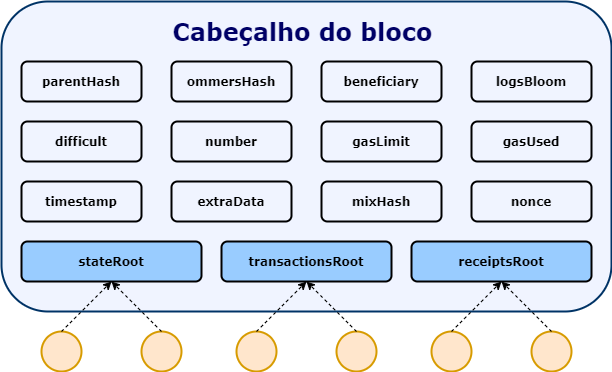
\includegraphics[scale=0.5]{figuras/eth_block_header.png}
 \fdireta{wood2014ethereum-yellow-paper}
\end{figure}

%Trie é a estrutura de dados para armazenar os dados da blockchain Ethereum (como os estados das contas)~\cite{wood2014ethereum-yellow-paper}. Uma árvore trie armazena pares de (chave, valor), facilitando a busca. O caminho da raiz até uma folha corresponde à chave, e os nós folha indicam um valor.

%---------------------------------%
\subsection{Validação} \label{tex:fund:ethereum:valida}

%Em uma blockchain, antes de um bloco ser adicionado à cadeia de blocos, este deve passar por um processo de validação por meio de um algoritmo de consenso distribuído. Este processo visa manter a integridade do histórico de transações executadas. Desta forma, cada bloco têm sua integridade verificada pelos nós da rede. Se a maioria dos nós atestarem a integridade do bloco, então este é adicionado à rede principal~\cite{consenso-xiao-2020, consenso-zhang2020analysis, consenso-Bouraga2021}.

Assim como na Bitcoin, na Ethereum os blocos também podem ser finalizados, transmitidos e recebidos em momentos distintos pelos mineradores, gerando assim um \textit{fork} com versões distintas do histórico de transações. Na Ethereum é utiliza uma variação do protocolo GHOST~\cite{sompolinsky2015ghost-original} para selecionar como parte da rede principal a ramificação com a maior dificuldade de bloco acumulada, enquanto que as demais sub-redes continuam existindo, mas sem fazer parte da rede principal~\cite{ethereum2014whitepaper}. 

Para cada ramificação, pode-se calcular a dificuldade acumulada, chamada também de ``o caminho mais pesado'', por meio do acesso às informações contidas no cabeçalho do último bloco adicionado. Como o cabeçalho contém a dificuldade de mineração do bloco, representada pelo campo \textit{difficult}, basta somar recursivamente o valor da dificuldade de mineração de todos os blocos da rede, exceto o bloco gênesis~\cite{wood2014ethereum-yellow-paper}. Na plataforma Etherscan~\footnote{\url{https://etherscan.io/}} são coletadas informações sobre todos os blocos e transações incluídos na blockchain Ethereum. Na Figura~\ref{fig:eth-block-difficulty} pode-se observar que, entre outras informações, há o campo \textit{Total Difficulty}, sublinhado em vermelho, seguido do valor da dificuldade acumulada na blockchain até o respectivo bloco.

\begin{figure}[htb]
 \caption{Dificuldade acumulada de um bloco na Ethereum}
 \label{fig:eth-block-difficulty}
 \centering
 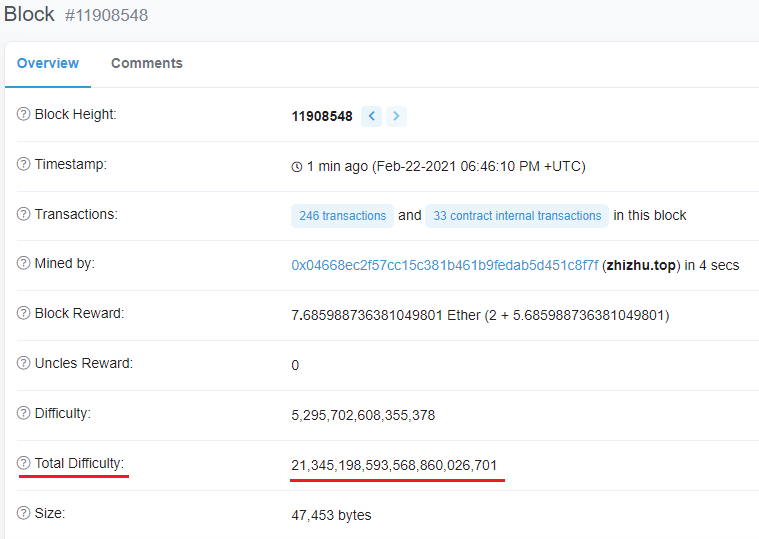
\includegraphics[scale=0.6]{figuras/block-eth-difficulty.png}
\end{figure}

%Em \cite{wang2019survey-consenso} tem uma explicação bem detalhada sobre o funcionamento do quebra-cabeça de hash da ethereum

%-------------------------------------------------------%
%\subsection{Máquina Virtual Ethereum}


%-------------------------------------------------------%
\subsection{Aplicações} \label{tex:fund:ethereum:aplica}

A tecnologia blockchain foi proposta inicialmente com o intuito de apoiar o desenvolvimento de criptomoedas como a Bitcoin. O êxito da Bitcoin chamou atenção tanto da academia quanto da indústria, e, posteriormente, outros tipos de criptomoedas e tecnologias baseadas na blockchain foram desenvolvidas. Como exposto por~\citeonline{swan2015blockchain-book} e~\citeonline{maesa2020blockchain3.0}, esses avanços são classificados como \textit{Blockchain 1.0}, \textit{2.0} e \textit{3.0}. Blockchains aplicados ao para gerenciamento de posse de criptomoedas integram um conjunto de aplicações classificado como \textit{Blockchain 1.0}. 

Com a introdução dos CIs, impulsionados principalmente pela blockchain Ethereum, possibilitou-se a implementação dos DApps. Desta forma, viabilizou-se o uso de sistemas descentralizados projetados para automatizar aplicações financeiras baseadas em criptomoedas, como OADs e sistemas de \textit{tokens}. Tais aplicações são baseadas na junção entre CIs e criptomoedas, e são definidas como \textit{Blockchain 2.0}~\cite{maesa2020blockchain3.0}. \textit{Blockchain 3.0} é o estágio evolucionário no qual a tecnologia não se limita apenas à aplicações financeiras, mas também à áreas como cuidados médicos, ciências, inteligência artificial, internet das coisas, governança descentralizada, entre outras~\cite{maesa2020blockchain3.0}. 

No decorrer desta seção são abordadas algumas áreas de aplicação da tecnologia blockchain baseadas na utilização de CIs, e são citados alguns exemplos de sistemas relacionados com as aplicações tratadas. Como a plataforma Ethereum faz parte do foco e do escopo deste trabalho, os exemplos citados são de aplicações desenvolvidas sobre a Ethereum, apesar de existirem outras blockchains que executam aplicações semelhantes.

\subsubsection*{\textbf{Sistemas de tokens}} 

Um \textit{token}  é um ativo digital e programável gerenciado por um CI para ser utilizado em um DApp ou algum projeto específico. \textit{Tokens} são similares às criptomoedas, porém, enquanto criptomoedas como Bitcoin e Ether possuem uma blockchain própria para sua mineração e gerenciamento, os \textit{tokens} são criados sobre a estrutura de uma blockchain já existente~\cite{angelo2020tokens}. \textit{Tokens} são usados para representar o direito sobre algo, de forma que esse direito é representado como um artefato digital, um processo conhecido como tokenização. Quando um artefato é tokenizado, é possível fracionar seu valor para quem se interessa em obter a posse, assim como já acontece com as criptomoedas tradicionais. Desta forma, facilita-se a entrada de investidores~\cite{angelo2020tokens}. 

Um exemplo de aplicação de \textit{tokens} são as \textit{stable coins}, moedas digitais cujo valor é lastreado de acordo com alguma moeda fiduciária ou fundos de investimentos já existentes. Projetos como o Tether~\footnote{Tether: Digital money for a digital age. \url{https://tether.to/}} e USD Coin~\footnote{USDC: the world's leading digital dollar stablecoin. ~\url{https://www.circle.com/en/usdc}} operam com as criptomoedas USDT e USDC, que são lastreadas pela cotação do dólar. Já o Pax Gold~\cite{paxgold-whitepaper}, opera por meio do  PAXG, uma versão tokenizada do ouro físico.

A facilidade para programação e o estabelecimento de padrões para criação de tokens, como o padrão ERC-20~\footnote{ERC-20 Token standard. ~\url{https://ethereum.org/en/developers/docs/standards/tokens/erc-20/}}, foram fundamentais para o estabelecimento deste tipo de ativo, que abrange diversas aplicações. Na plataforma Etherscan~\footnote{Etherscan. Token Traker. \url{https://etherscan.io/tokens}} pode-se consultar uma lista de \textit{tokens} criados, na qual, no momento da escrita deste trabalho, foram encontrados 362.745, considerando apenas aqueles escritos no padrão ERC-20.

\subsubsection*{\textbf{Organizações Autônomas Descentralizadas}} 

Uma OAD é uma organização desenvolvida por meio da tecnologia blockchain que pode ser gerida de forma autônoma, sem a necessidade de confiar em uma autoridade central ou estruturas hierárquicas~\cite{wang2019DAO-survey}. Em uma OAD, todas as regras operacionais e de gerenciamento são programadas em um CI e gravadas em uma blockchain. Assim, protocolos de consenso e \textit{tokens} são utilizados como incentivo para estimular a autonomia operacional e governamental das organizações. Por meio da implantação de uma OAD, espera-se abolir modelos de gerenciamento tradicionais baseados em hierarquia, além de reduzir os custos das organizações com comunicação, gerenciamento e colaboração~\cite{wang2019DAO-survey}.

Em 2016, foi lançado o primeiro OAD, chamado de \textit{The DAO} (sigla para \textit{Decentralized Autonomous Organization}), o maior projeto de \textit{crowdfunding} da época~\footnote{\url{https://bitcoinmagazine.com/business/the-dao-raises-more-than-million-in-world-s-largest-crowdfunding-to-date-1463422191}}, que em pouco tempo arrecadou cerca de 150 milhões de dólares. Por meio do \textit{The DAO}, propostas de investimento eram submetidas e os participantes compravam \textit{tokens} que davam direito de participação na aprovação das propostas, assim como receber parte dos lucros gerados~\cite{wang2019DAO-survey}. Após o \textit{The DAO} outras OADs surgiram, como a \textit{Aragon}~\footnote{Aragon: Next-level communities run on Aragon. ~\url{https://aragon.org/}} e a \textit{Steemit}~\footnote{Steemit. ~\url{https://steemit.com/}}. 

%A \textit{Aragon} é uma plataforma que oferece aos usuários uma infraestrutura para criação e gerenciamento de vários tipos de OADs. A \textit{Steemit} é uma plataforma de mídias sociais baseada em blockchain que, por meio de um sistema de tokens, usuários são recompensados pela criação e curadoria de conteúdos.  

%Por se tratarem de plataformas com grande capacidade de arrecadação financeira, as OADs tornaram-se alvo de ataques~\cite{atzei2017survey-attacks-sok}. Em junho 2016 ocorreu o caso conhecido como \textit{The DAO Attack}, no qual um participante malicioso explorou uma falha no contrato e transferiu cerca de 3,6 milhões de Ether para sua conta, o equivalente a 50 milhões de dólares~\cite{siegel-dao-attack}. Este caso teve grande repercussão e chamou a atenção da academia e da indústria, impulsionando estudos e estratégias para detecção e prevenção de vulnerabilidades em CIs~\cite{chen2020survey-ethereum-acm, liu2019survey-ieeeaccess}.

\subsubsection*{\textbf{Cuidados médicos e serviços de saúde}}

%Com a ampla difusão da informatização de processos em diversas áreas e do acesso à \textit{internet}, aliados à popularização de \textit{smartphones} e computadores pessoais, um dos maiores problemas enfrentados diz respeito à proteção dos dados pessoais dos usuários. Entre esses dados pessoais estão as informações de serviços de saúde. O histórico médico contém dados sensíveis de pacientes, que precisam ser compartilhados com médicos, farmácias, seguradoras, e outras partes interessadas da área da saúde. Ao mesmo tempo, essas dados devem ser protegido contra acessos indevidos e manipulados corretamente pelos profissionais da área, que muitas vezes não têm conhecimento técnico para lidar com os dados de forma segura.  Além da preocupação com a proteção dos dados, também há falta de padronização do formato desses dados, que podem enfrentar incompatibilidade no compartilhamento entre instituições médicas, profissionais da saúde, e outras partes interessadas~\cite{maesa2020blockchain3.0}. Outro problema na área da saúde é à falsificação e adulteração da composição de medicamentos. De acordo com a Organização \sigla{OMS}{Organização Mundial da Saúde}, em 2017, 1 em cada 10 medicamentos nos países em desenvolvimento eram falsificados ou de baixa qualidade~\cite{oms2017medicamentos}. Diante desses problemas, diversas soluções foram propostas utilizando como base a tecnologia blockchain, que possui potencial para transformar a área de cuidados médicos e serviços de saúde~\citeonline{mcghin2019blockchain-survey-health, erikson2020survey-health}. 

Na área da saúde, a tecnologia blockchain pode oferecer uma infraestrutura adequada para integração de dados de prontuários médicos, e outros benefícios proporcionados pela integridade e imutabilidade dos dados. Uma proposta que utiliza CIs e a estrutura da Ethereum é o sistema MedRec~\cite{ekblaw2016case-medrec}, utilizado para gerenciamento de registros de prontuário eletrônicos. O MedRed permite que pacientes consultem suas informações de forma acessível e oferece uma estrutura modular que facilita a interoperabilidade com sistemas já existentes, além de gerenciar questões como autenticação, confidencialidade, contabilidade e compartilhamento de dados~\cite{ekblaw2016case-medrec}. Outros exemplos de aplicações da blockchain na área da saúde são relatados nos trabalhos de ~\citeonline{mcghin2019blockchain-survey-health} e ~\citeonline{erikson2020survey-health}.

%%%%%%%
%%%%% mais p frente falar tbm do uso com IA e IoT

%--------------------------------------------%
\subsection{Arquitetura em camadas} \label{tex:fund:ethereum:camadas}

% Em \citeonline{fan2020performance} são descrita 5 camadas, com a EVM em uma camada separada de execução

A blockchain Ethereum foi projetada sobre uma série de conceitos, protocolos e procedimentos, que dependem de recursos computacionais e tecnológicos para funcionar. Esse conjunto de elementos compõem a arquitetura da Ethereum. Em seu trabalho, \citeonline{chen2020survey-ethereum-acm} dividem essa arquitetura em quatro camadas: aplicação; dados; consenso; e rede. 

A arquitetura em camadas conta também com elementos presentes no ambiente, relacionados com recursos tecnológicos e infraestrutura, como exposto na Figura~\ref{fig:eth-arquitetura}. Na camada de aplicação estão as contas, que podem ser CPEs ou CCs, os CIs, e a MVE, responsável pela execução do \textit{bytecode} gerado na compilação do contrato. A camada de dados consiste nas informações geradas ao longo da execução dos contratos, como transações e \textit{logs} de eventos, e no armazenamento destas, que são acessadas por meio dos blocos. Os mecanismos para validação dos blocos estão incluídos na camada de consenso, no qual um algoritmo de consenso e uma política de incentivos é utilizada para motivar os mineradores a agirem de forma honesta. A camada de rede é a responsável pela comunicação entre os participantes da rede, possibilitando a descoberta de novos nós e a propagação e verificação das informações, essencial para que cada nó possa manter seu histórico de transações atualizado~\cite{chen2020survey-ethereum-acm}.    

\begin{figure}[htb]
 \caption{Arquitetura da blockchain Ethereum e seu ambiente de execução}
 \label{fig:eth-arquitetura}
 \centering
 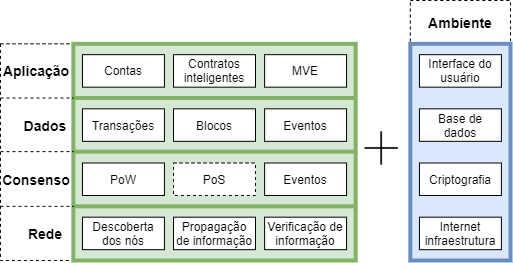
\includegraphics[scale=0.5]{figuras/ethereum_arquitetura.png}
 \fdireta{chen2020survey-ethereum-acm}
\end{figure}

Cada camada depende de componentes do ambiente de execução das aplicações, como uma interface \textit{web} para interação dos usuários com as aplicações, uma base de dados para armazenamento dos dados da blockchain, mecanismos criptográficos para apoiar os protocolos de consenso, e o serviço de \textit{Internet} que apoia as tarefas da camada de rede~\cite{chen2020survey-ethereum-acm}.

Na Figura~\ref{fig:eth-arquitetura}, nota-se que, na camada de consenso, o retângulo contendo o algoritmo PoS está com o contorno pontilhado. Isto deve-se ao fato da rede Ethereum 2.0, que opera com o algoritmo de consenso PoS, estar em fase inicial de implementação. Futuramente, de acordo com o planejamento do projeto, espera-se que a Ethereum seja englobada pela Ethereum 2.0.

Os contratos inteligentes, que integram a camada de aplicação, são discutidos adiante, na Seção~\ref{tex:fund:ethereum:smartc}. Além disso, também são apresentadas algumas vulnerabilidades presentes nas aplicações que executam sobre a Ethereum. Apesar de haverem diversas vulnerabilidades em todas as camadas~\cite{chen2020survey-ethereum-acm}, na Seção~\ref{tex:fund:ethereum:vuln-ataques} são expostas apenas vulnerabilidades e ataques relacionados com a camada de aplicação da Ethereum, pois são o foco desta pesquisa.  

%%%%%% mais p frente, usar tbm o trabalho ~\cite{zhang2019blockchain-security-acmcs} na fundamentação

\section{Contratos inteligentes} \label{tex:fund:ethereum:smartc}

No trabalho de ~\citeonline{szabo1997smart-contract} foi proposta pela primeira vez a ideia de um CI cujas cláusulas são escritas em programas de computador e executadas automaticamente sem a necessidade de confiar em uma terceira parte reguladora. Anos depois, por meio da tecnologia blockchain, os CIs puderam ser de fato implementados, impulsionados por plataformas como Ethereum, Hyperledger Fabric, Corda e Stellar~\cite{overview-smartcontracts2020zheng}.

Para desenvolvimento de um CI, as cláusulas contratuais estabelecidas em comum acordo entre as partes envolvidas são expressas por meio de programas de computador executáveis. Esses programas são normalmente escritos em linguagens de programação de alto nível, como a linguagem Solidity~\footnote{\url{https://readthedocs.org/projects/solidity/}}. Na plataforma Ethereum, independente da linguagem, os CIs são sempre convertidos em um \textit{bytecode}, uma linguagem de baixo nível que é executada na MVE.

Contratos escritos na linguagem Solidity são similares à objetos. Cada contrato possui atributos e funções que podem ter seus controles de acesso definidos por modificadores. O controle lógico das condições estabelecidas pelas cláusulas podem ser definidos por meio de estruturas de controle, como \textit{if}, \textit{if-else}, \textit{for}, etc. Um exemplo de contrato escrito na linguagem Solidity é exposto na Figura~\ref{fig:exemplo-contrato-solidity}. Neste exemplo~\footnote{Exemplo obtido da documentação da linguagem Solidity, disponível em: \url{https://docs.soliditylang.org/en/v0.5.9/introduction-to-smart-contracts.html}}, a conta que implementa o contrato pode atribuir algum saldo para si ou para outras contas, e esses valores atribuídos podem ser transferidos para outras contas.

\begin{figure}[htb]
 \caption{Contrato escrito na linguagem Solidity para atribuição e transferência de saldo}
 \label{fig:exemplo-contrato-solidity}
 \centering
 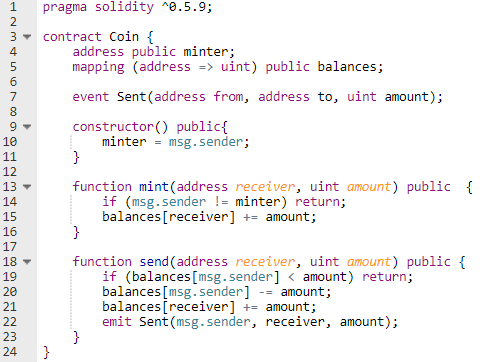
\includegraphics[scale=0.7]{figuras/exemplo_codigo_solidity.png}
\end{figure}

Em seu trabalho, ~\citeonline{overview-smartcontracts2020zheng} descreveram a utilização dos CIs como um ciclo de vida que consiste em quatro fases: criação; implantação; execução; e conclusão. Cada fase é descrita como segue:
\begin{enumerate}
    \item \textbf{Criação:} Essa primeira fase se inicia com a negociação entre as partes envolvidas para definição das obrigações, direitos e proibições que devem ser expressas no contrato. Em seguida, desenvolvedores e engenheiros de \textit{software} descrevem esse acordo para alguma linguagem de programação para CIs, um processo para por etapas de projeto, implementação e validação. A criação de CIs é uma etapa interativa que pode envolver a participação de vários profissionais, como investidores, advogados e engenheiros de \textit{software};
    \item \textbf{Implantação:} Consiste em implantar o contrato compilado na blockchain, que então não pode mais ser modificado. A implantação é feita por meio de plataformas como a Go Ethereum~\footnote{\textit{Go Ethereum: Official Golang implementation of the Ethereum protocol}. \url{https://github.com/ethereum/go-ethereum}}, que opera sobre a blockchain Ethereum. Nesta etapa, os envolvidos podem ter uma parcela de seus bens digitais bloqueados. Esse bem digital pode ser uma quantidade de Ether dada como garantia de uma transferência, por exemplo. Assim, as partes envolvidas são identificadas por meio de suas carteiras digitais; 
    \item \textbf{Execução:} Após a implantação, a execução do contrato é monitorada e avaliada. Conforme as condições estabelecidas são atingidas, operações e funções expressas no contrato são automaticamente executadas, o que gera um fluxo de transações que são executadas e validadas pelos mineradores;
    \item \textbf{Conclusão:} Depois que um contrato é executado, o estado das contas envolvidas é atualizado. Logo, as transições e os dados de atualização dos estados são gravados na blockchain, as transferências entre as contas são concretizadas e os bens digitais das partes envolvidas são desbloqueados. Por fim, o ciclo de vida de um CI é concluído. 
\end{enumerate}

\begin{figure}[htb]
 \caption{Ciclo de vida de um CI baseado em 4 fases: criação, implantação, execução e conclusão}
 \label{fig:contrato-ciclo-de-vida}
 \centering
 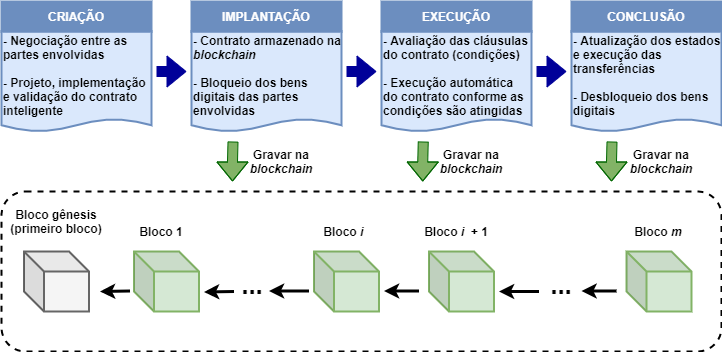
\includegraphics[scale=0.6]{figuras/contrato_ciclo_de_vida.png}
 \fdireta{overview-smartcontracts2020zheng}
\end{figure}

O ciclo de vida dos CIs é ilustrado na Figura~\ref{fig:contrato-ciclo-de-vida}. Nota-se que, durante as fases de implantação, execução e conclusão, uma série de transações são geradas, transmitidas, validadas e gravadas na blockchain, proporcionando a rastreabilidade e auditabilidade do contrato~\cite{overview-smartcontracts2020zheng}.

Devido à imutabilidade da blockchain, um contrato implementado não pode mais ser alterado. Esta propriedade agrega integridade à tecnologia blockchain, mas também ressalta a importância da implementação de contratos livres de erros e de acordo com boas práticas, já que vulnerabilidades presentes nos contratos podem torná-los alvos de ataques.

A seguir, na Seção~\ref{tex:fund:ethereum:vuln-ataques} são abordadas algumas das vulnerabilidades já encontradas em CIs e ataques que ocorreram por meio da exploração dessas vulnerabilidades.  

%-----------------------------------------------------------------------%
\subsection{Vulnerabilidades e ataques} \label{tex:fund:ethereum:vuln-ataques}

Aplicações desenvolvidas por meio de CIs, como os DApps e as OADs, costumam envolver transferências e gerenciamento de grandes quantidades de bens digitais, e isso tornou-os alvos de uma série de ataques que exploraram vulnerabilidades encontradas no código desses contratos~\cite{atzei2017survey-attacks-sok, liu2019survey-ieeeaccess, chen2020survey-ethereum-acm}. O primeiro desses ataques ocorreu em 2016 sobre a OAD de \textit{crowdfunding} \textit{The DAO}, no caso conhecido como \textit{The DAO Attack}. Na ocasião, um participante malicioso explorou uma falha no contrato e transferiu cerca de 3,6 milhões de Ether para sua conta, o equivalente a 50 milhões de dólares~\cite{siegel-dao-attack}. Este caso teve grande repercussão e chamou a atenção da academia e indústria, motivando estudos e estratégias para detecção e prevenção de vulnerabilidades em CIs~\cite{chen2020survey-ethereum-acm, liu2019survey-ieeeaccess}.

Há vários fatores que tornam a implementação de CIs propícios a erros. Segundo ~\citeonline{atzei2017survey-attacks-sok}, parte desses erros são ocasionados pelo desalinhamento que há entre a semântica da linguagem Solidity e a intuição dos desenvolvedores. Apesar de alguns elementos em Solidity serem similares aos encontrados em outras linguagens, como funções, exceções e modificadores de acesso, estes não são implementados da mesma forma.

No decorrer desta seção são discutidas algumas vulnerabilidades conhecidas, assim como os ataques resultantes da exploração destas. Ao final, outras vulnerabilidades encontradas na literatura são listadas e brevemente descritas.

%Desde os primeiros casos notórios de ataques, como o ataque ao The DAO~\cite{siegel-dao-attack}, mencionado na Seção~\ref{tex:fund:ethereum:app:oad}, diversos trabalhos foram desenvolvidos com o intuito de listar e classificar os ataques e as vulnerabilidades explorados em CIs, e também relatar os esforços despendidos na mitigação dessas ameaças. 

%No trabalho de~\citeonline{chen2020survey-ethereum-acm} são identificadas 40 vulnerabilidades relacionadas com a blockchain Ethereum. Cada vulnerabilidade encontra-se em uma das camadas da arquitetura da Ethereum, a qual é ilustrada na Figura~\ref{fig:eth-arquitetura}. Das vulnerabilidades identificadas, 26 estão na camada de aplicação, que engloba as contas, os CIs e a MVE. Destas, 14 estão associadas à programação dos CIs. Em outro trabalho, desenvolvido por~\citeonline{atzei2017survey-attacks-sok}, são identificadas 6 vulnerabilidades em contratos escritos na linguagem Solidity, sobre as quais 6 ataques foram realizados. Algumas dessas vulnerabilidades, assim como os respectivos ataques, são descritos no decorrer desta Seção.

%%%%%%%%%%%%
%- No trabalho de \cite{wang2019contractguard-19} as vulnerabilidades são abordadas sob a perspectiva de \textbf{ataques de intrusão}, embora sejam as mesmas abordadas em outros trabalhos.
%- Nos trabalhos de \cite{wang2019detecting-nondeterministic-26} e \cite{kolluri2019exploiting-37} a execução de CIs e das transações e as vulnerabilidades decorrentes destas são analisadas sob a perspectiva de não-determinismo, isto é, a execução de uma transação possui comportamento não determinístico.

\subsubsection*{\textbf{Reentrância}}

A reentrância foi a vulnerabilidade explorada contra a OAD \textit{The DAO}, mencionada na Seção~\ref{tex:fund:ethereum:aplica}, no ataque conhecido como \textit{The DAO Attack}. Essa vulnerabilidade ocorre quando o contrato de um receptor externo invoca novamente uma função do tipo \textit{callback} de outro contrato antes que este termine de executar essa função. Quando um contrato vulnerável contém uma função \textit{callback}, um contrato externo pode invocá-la sucessivas vezes até esgotar qualquer saldo contido no contrato~\cite{chen2020survey-ethereum-acm, sayeed2020smart-attacks-ieee}. 

\begin{figure}[!htb]
 \caption{Exemplo simplificado do \textit{The DAO Attack}}
 \label{fig:reentrancia-exemplo}
 \centering
 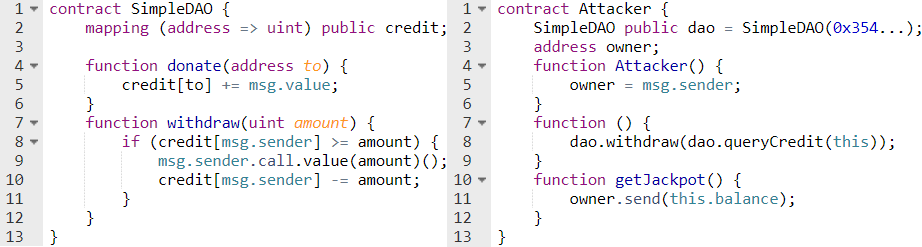
\includegraphics[scale=0.65]{figuras/reentrancia-exemplo.png}
 \fdireta{atzei2017survey-attacks-sok}
\end{figure}

É apresentada na Figura~\ref{fig:reentrancia-exemplo} uma versão simplificada desenvolvida por~\citeonline{atzei2017survey-attacks-sok} do contrato \textit{The DAO} e de um contrato malicioso similar ao que executou o ataque~\footnote{Esse código é desenvolvido na linguagem Solidity v0.4.2.}~\footnote{Uma análise completa do \textit{The DAO Attack} é fornecida em \url{https://hackingdistributed.com/2016/06/18/analysis-of-the-dao-exploit/}}. Neste exemplo, o contrato \texttt{Attacker} é capaz de explorar a vulnerabilidade e transferir todos os fundos do contrato \texttt{SimpleDAO} para a conta de seu criador. Após a implantação do contrato \texttt{Attacker}, o primeiro passo do ataque é a publicação do contrato (linha de código 2), na qual é criada uma instância do \texttt{SimpleDAO} com o endereço da CC do \texttt{Attacker}. Então, o usuário malicioso utiliza sua CPE para doar algum Ether para o contrato \texttt{Attacker} por meio de uma chamada à função \texttt{donate}, e logo após invoca a função do tipo \textit{fallback}~\footnote{\textit{Fallback} é uma função sem argumentos e sem retorno que é executada na invocação de um contrato quando nenhuma outra função corresponde ao identificador de função fornecido, ou quando não é fornecido nenhum dado.} (linha de código 7 do \texttt{Attacker}). Em seguida, a função \textit{fallback} invoca a função \texttt{withdraw}, e o Ether é transferido para o \texttt{Attacker}. Da forma como é usada, a função \texttt{call} (linha 9 do \texttt{SimpleDAO}), que é uma função \textit{callback}, tem como efeito uma nova invocação da função \textit{fallback} do \texttt{Attacker}, que, maliciosamente, executa a função \texttt{withdraw} novamente. Como a execução da \texttt{withdraw} foi interrompida antes do valor \texttt{credit[msg.sender]} ser atualizado, a condição verificada na linha 8 tem êxito novamente. Consequentemente, o \texttt{SimpleDAO} realiza a transferência de Ether de novo, invoca outra vez a função \textit{callback} e assim sucessivamente, até ocorrer um dos seguintes eventos: (i) todo o \textit{gas} é utilizado; ou (ii) a pilha de chamadas da MVE é totalmente preenchida; ou (iii) o saldo do \texttt{SimpleDAO} é zerado.

Esta vulnerabilidade poderia ter sido evitada se um dos seguintes procedimentos tivessem sido adotados~\cite{consensys2021bestpractices}: (i) garantir que as variáveis do estado do contrato (e.g., \texttt{credit[msg.sender]}) são atualizadas antes de outro contrato ser invocado; (ii) introduzir uma trava \textit{mutex} ao estado do contrato para assegurar que apenas o dono da trava pode alterar o estado; (iii) utilizar o método de transferência \texttt{transfer} para enviar Ether à outros contratos, pois este método possui um baixo limite de \textit{gas} definido para sua execução. 

Apesar dos danos do \textit{The DAO Attack} terem sido revertidos, isso causou uma divisão entre os mineradores da Ethereum. A maior parte dos mineradores concordaram em reverter os danos por meio de um \textit{hard fork}, um procedimento no qual é feita uma bifurcação na cadeia de blocos, que neste caso, foi referente ao momento anterior ao ataque. Após o \textit{hard fork}, a cadeia de blocos principal da Ethereum continuou a partir do bloco 1920000~\footnote{\textit{Hard Fork Completed}. \url{https://blog.ethereum.org/2016/07/20/hard-fork-completed/}}, enquanto que a outra cadeia foi continuada pelos mineradores que não concordaram com a decisão, e foi denominada como Ethereum Classic~\footnote{Ethereum Classic. \url{https://ethereumclassic.org/}}.  

\subsubsection*{\textbf{Delegatecall Injection}}

Para facilitar o reuso de código, a MVE dispõe do código de operação (do inglês, \textit{opcode}) \texttt{delegatecall}, usado para inserir o \textit{bytecode} de um contrato no \textit{bytecode} de outro contrato, que irá executá-lo por meio de uma chamada. Quando isso ocorre, o contrato que é chamado pode alterar as variáveis de estado do contrato que o invocou. Essa característica torna este último contrato vulnerável à ação de contratos maliciosos que, quando chamados, podem causar alterações para obter benefícios e transferir \textit{tokens} para sua conta~\cite{chen2020survey-ethereum-acm}.

O primeiro ataque a explorar essa vulnerabilidade ocorreu contra a \textit{Parity Multsignature Wallet} (ou apenas \textit{Parity Wallet}), uma carteira multi-assinatura. Para se autorizar uma transação convencional de Ether, o remetente deve assinar a transação com sua chave privada. Na Ethereum, uma carteira multi-assinatura é um CI que requer múltiplas chaves privadas para desbloquear uma carteira e autorizar transferências. Em 2017, uma vulnerabilidade em uma chamada \texttt{delegatecall} foi explorada, e cerca de 31 milhões de dólares em Ether foi subtraído da \textit{Parity Multsignature Wallet}~\cite{chen2020survey-ethereum-acm}.

\begin{figure}[!htb]
 \caption{Exemplo simplificado dos contratos da \textit{Parity Multsignature Wallet}}
 \label{fig:parity-wallet}
 \centering
 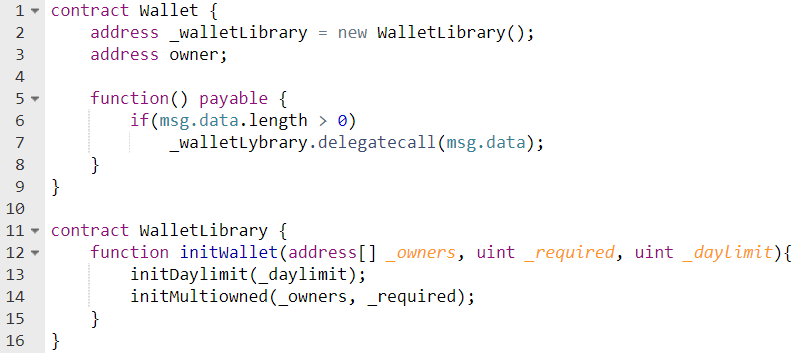
\includegraphics[scale=0.65]{figuras/parity-wallet.png}
 \fdireta{chen2020survey-ethereum-acm}
\end{figure}

Uma versão simplificada do contrato explorado é exposta na Figura~\ref{fig:parity-wallet}. A \textit{Parity Multsignature Wallet} consiste em dois contratos. O primeiro, \texttt{WalletLibrary}, é utilizado como uma biblioteca, e implementa as principais funções da carteira. O segundo, \texttt{Wallet}, contém uma referência (i.e., \texttt{\_walletLibrary}) dentro de uma função \textit{fallback} que encaminha todas as chamadas de função não correspondidas para o contrato \texttt{WalletLibrary} por meio de uma chamada \texttt{delegatecall} (linha 7). No ataque ocorrido, o atacante assumiu a posse do contrato \texttt{Wallet} após enviar uma transação com o campo \texttt{msg.data} contendo \texttt{iniWallet()} como a função a ser chamada. Como essa função não existe no contrato \texttt{Wallet}, a função \textit{fallback} foi invocada e a inicialização da carteira foi feita pela função \texttt{initWallet} em \texttt{WalletLibrary}, a qual substituiu os endereços originais de posse do contrato pelo endereço do atacante especificado em \texttt{msg.data}. Uma vez obtida a posse do contrato, o atacante transferiu 31 milhões de dólares em Ether para sua conta. Esta vulnerabilidade pode ser evitada se o contrato a ser compartilhado por meio de uma \texttt{delegatecall} (e.g., o contrato \texttt{WalletLibrary}) for declarado como uma biblioteca, que tem seu estado estático (\textit{stateless}) e não como um contrato, que possui um estado dinâmico (\textit{statefull})~\cite{chen2020survey-ethereum-acm}. Na linguagem Solidity, isto é feito usando a palavra-chave \texttt{library}~\cite{knownattacks2018}.

\subsubsection*{\textbf{Contrato suicida}}

Um contrato pode ser ``morto'' pelo dono do contrato, ou alguma terceira parte confiável, por meio dos métodos \texttt{suicide} ou \texttt{selfdestruct}. Quanto isso acontece, o \textit{bytecode} e o armazenamento do contrato é deletado. A vulnerabilidade contrato suicida, também conhecida como suicídio desprotegido, acontece quando uma autenticação inadequada permite que algum invasor tome posse do contrato e execute a função para matar o contrato~\cite{chen2020survey-ethereum-acm}. 

\begin{figure}[!htb]
 \caption{Contrato da \textit{Parity Wallet}, corrigido após o primeiro ataque}
 \label{fig:parity-corrigido}
 \centering
 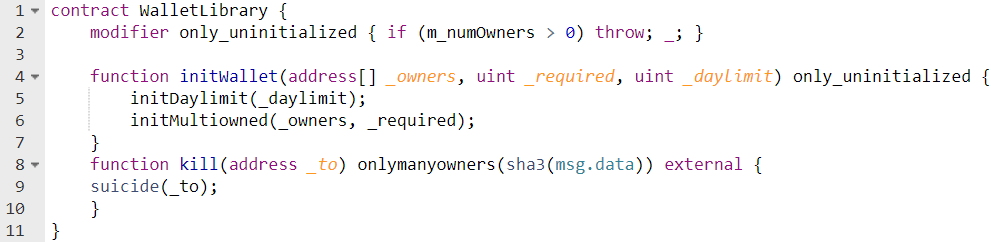
\includegraphics[scale=0.65]{figuras/parity-corrigido.png}
 \fdireta{paritywallet2017attack}
\end{figure}

Essa vulnerabilidade foi explorada em um segundo ataque efetuado contra a \textit{Parity Wallet}. Como resposta ao primeiro ataque contra a \textit{Parity Wallet}, foi adicionado um modificador, \texttt{only\_uninitialized}, como ilustrado no Figura~\ref{fig:parity-corrigido}. Desta forma, pretendia-se proteger a função \texttt{initWallet()} de forma que uma reinicialização da \texttt{Wallet} por meio da chamada \texttt{delegatecall} teria como resposta o disparo de uma exceção, e então seria rejeitada pelo modificador. Porém, o próprio contrato \texttt{WalletLibrary} foi deixado como não inicializado, e o invasor pôde passar pelo modificador \texttt{only\_uninitialized} e se autodeclarar o dono do  contrato. Assim que assumiu o controle da biblioteca, o invasor invocou o método \texttt{suicide} para matar o contrato. Por consequência, todas as carteiras criadas pelo contrato \texttt{Wallet} que dependem da biblioteca foram inutilizadas, o que causou o bloqueio permanente de 280 milhões de dólares em Ether associados às carteiras~\cite{chen2020survey-ethereum-acm, destefanis2018smart-parity-wallet}.

%Monitoramento em tempo real é pouco explorado \cite{chen2020survey-ethereum-acm} 

% SE DER TEMPO, incluir sessão sobe a execução do bytecode de um contrato na Ethereum Virtual Machine

\subsubsection*{\textbf{Outras vulnerabilidades}}

As vulnerabilidades discutidas nesta seção são o foco desta pesquisa. Entretanto, existem diversas vulnerabilidades encontradas na literatura, e algumas delas são listadas e brevemente descritas na Tabela~\ref{tab:vulnerabilidades}. Diante dos ataques efetuados que exploraram vulnerabilidades nos CIs e suas consequências, uma série de pesquisas foram realizadas nos últimos anos com foco na verificação de CIs e detecção de vulnerabilidades, nas quais diversas técnicas têm sido empregadas~\cite{chen2020survey-ethereum-acm, almakhour2020verification-survey, liu2019survey-ieeeaccess, singh2020survey-vulnerabilities-elsevier}. Algumas dessas técnicas são discutidas a seguir na Seção~\ref{tex:fund:verificacao}.

\begin{table}[!ht]
\centering
\fontsize{9.5pt}{10.25pt}\selectfont
\caption{Tipos de vulnerabilidades em contratos inteligentes}
\label{tab:vulnerabilidades}
\begin{tabular}{|l|l|} 
\hline
\textbf{Vulnerabilidade}                                                             & \textbf{Descrição}                                                                                                                                                                                                                                                                                                                                                                                                                                                                                                                                                                                       \\ 
\hline
\begin{tabular}[c]{@{}l@{}}Ataque de profundidade da\\pilha de chamadas\end{tabular} & Acontece quando é excedido o limite de chamadas ao~método de um contrato.                                                                                                                                                                                                                                                                                                                                                                                                                                                                                                                                \\ 
\hline
\begin{tabular}[c]{@{}l@{}}Ataque DoS com operações\\ilimitadas\end{tabular}         & \begin{tabular}[c]{@{}l@{}}Essa vulnerabilidade é resultante de programação~imprópria com operações ilimitadas em \\um contrato, que podem entrar em \textit{loop} indefinidamente.\end{tabular}                                                                                                                                                                                                                                                                                                                                                                                                         \\ 
\hline
Autenticação com~\texttt{tx.origin}                                                           & \begin{tabular}[c]{@{}l@{}}Ocorre quando um contrato utiliza~\texttt{tx.origin}~para~autenticação do dono ou administrador do\\contrato ao invés de usar msg.sender. Assim, autenticação pode ser comprometida por~um \\ataque~\textit{phishing}.\end{tabular}                                                                                                                                                                                                                                                                                                                                                             \\ 
\hline
Bloqueio de Ether                                                                    & \begin{tabular}[c]{@{}l@{}}Os fundos do contrato ou o saldo em ether são~travados indefinidamente, isto é, o CI pode\\receber Ether mas não pode enviar.\end{tabular}                                                                                                                                                                                                                                                                                                                                                                                                                                    \\ 
\hline
Consumo de~\textit{gas}~ineficiente                                                           & Consumo de~\textit{gas}~desnecessário na execução do~código do contrato.                                                                                                                                                                                                                                                                                                                                                                                                                                                                                                                                          \\ 
\hline
Contrato pródigo                                                                     & O contrato pode liberar fundos ou saldo em Ether para usuários~arbitrários.                                                                                                                                                                                                                                                                                                                                                                                                                                                                                                                              \\ 
\hline
Contrato~\textit{honeypot}                                                           & \begin{tabular}[c]{@{}l@{}}Decorre da inserção intencional de vulnerabilidades em um CI para atrair usuários \\maliciosos, que depositam Ether com a intenção de explorar o contrato, mas não \\conseguem recuperar a quantia depositada.\end{tabular}                                                                                                                                                                                                                                                                                                                                                   \\ 
\hline
Controle de acesso vulnerável                                                        & \begin{tabular}[c]{@{}l@{}}Quando uma função que lida com informações sensíveis (e.g., um método construtor) permite\\o acesso de usuários arbitrários.\end{tabular}                                                                                                                                                                                                                                                                                                                                                                                                                                     \\ 
\hline
\begin{tabular}[c]{@{}l@{}}Dependência de informação\\do bloco\end{tabular}          & \begin{tabular}[c]{@{}l@{}}Também conhecido como dependência de variável previsível, ocorre quando um contrato\\utiliza informação de um bloco para disparar ações, ou como semente para geração de\\números aleatórios. Um minerador malicioso pode se aproveitar disso para obter benefícios.~\end{tabular}                                                                                                                                                                                                                                                                                            \\ 
\hline
\begin{tabular}[c]{@{}l@{}}Dependência de ordem da\\transação\end{tabular}           & Ordem das transações inconsistente em relação~ao momento da invocação.                                                                                                                                                                                                                                                                                                                                                                                                                                                                                                                                   \\ 
\hline
Dependência de~\textit{timestamp}                                                    & \begin{tabular}[c]{@{}l@{}}Ocorre quando um contrato que utiliza o~\textit{timestamp}~de um bloco como parte da condição para\\acionar~uma operação crítica (e.g. envio de Ether) é~explorado por um minerador malicioso.\end{tabular}                                                                                                                                                                                                                                                                                                                                                                   \\ 
\hline
Desordem de exceções                                                                 & \begin{tabular}[c]{@{}l@{}}Se dois ou mais contratos interagem entre si, então a função de um contrato pode depender\\da execução de uma função em outro contrato, e assim sucessivamente, criando uma corrente\\de chamadas de funções aninhadas. Caso a invocação de alguma função for feita por meio \\das chamadas \texttt{address.call()}, \texttt{address.delegatecall()}, ou \texttt{address send()} e ocorrer\\um erro nesta função, as transações não serão revertidas e os outros contratos não estarão cientes\\do erro, o que pode resultar em alterações inesperadas no estado dos contratos envolvidos.\end{tabular}  \\ 
\hline
Divisão por zero                                                                     & É um erro aritmético que ocorre quando há uma divisão por zero ou módulo zero.                                                                                                                                                                                                                                                                                                                                                                                                                                                                                                                           \\ 
\hline
Endereço curto                                                                       & \begin{tabular}[c]{@{}l@{}}A MVE não verifica a validade de endereços. Desta forma, se o tamanho de uma variável\\\texttt{address} na chamada de uma função for menor do que o esperado, então a quantidade de~\textit{bytes}\\no argumento da função também será menor do que o esperado, e os \textit{bytes }restantes serão\\preenchidos com zeros hexadecimais, o que pode alterar o valor dos parâmetros.\end{tabular}                                                                                                                                                                                       \\ 
\hline
Exceções não tratadas                                                                & \begin{tabular}[c]{@{}l@{}}Ocorre quando uma exceção é disparada em um CI por~meio da chamada de outro contrato e\\não é tratada~devidamente por aquele que fez a chamada.\end{tabular}                                                                                                                                                                                                                                                                                                                                                                                                                  \\ 
\hline
\begin{tabular}[c]{@{}l@{}}Chamada externa não\\verificada\end{tabular}              & O valor de retorno de uma chamada à outro contrato não é verificado.                                                                                                                                                                                                                                                                                                                                                                                                                                                                                                                                     \\ 
\hline
Integer \textit{overflow}~e~\textit{underflow}                                                         & \begin{tabular}[c]{@{}l@{}}Um~\textit{overflow}/\textit{underflow}~pode ocorrer quando são~executadas operações de adição, subtração,\\ou~armazenamento da entradas do usuário sobre~variáveis inteiras com limitações de valor.\end{tabular}                                                                                                                                                                                                                                                                                                                                                                              \\ 
\hline
Gasto de~\textit{gas}~descontrolado                                                           & Ocasiona um consumo de~\textit{gas}~desnecessário na execução do~código do contrato.                                                                                                                                                                                                                                                                                                                                                                                                                                                                                                                              \\
\hline
\end{tabular}
\fdireta{fu2019critical-02, chen2020survey-ethereum-acm, lu2019neucheck-63, huang2021hunting-53, ashraf2020gasfuzzer-51, jiang2018contractfuzzer-18, torres2018osiris-65}
\end{table}

%-------------------------------------------------------------
\section{Verificação e validação} \label{tex:fund:verificacao}

Grande parte das vulnerabilidades encontradas em CIs escritos em Solidity poderiam ter sido evitadas com a ajuda de análise formal e verificação desses contratos antes de serem implantados na blockchain~\cite{singh2020survey-vulnerabilities-elsevier, chen2020survey-ethereum-acm}. Porém, as linguagens de domínio específico encontradas no estado da arte, como Solidity, não foram desenvolvidas com o intuito de serem verificadas formalmente, fazendo disso uma tarefa desafiadora. Além disso, Solidity não é uma linguagem perfeita para escrever CIs, já que é vulnerável à certos riscos~\footnote{Solidity. \textit{Security Considerations}.\url{https://docs.soliditylang.org/en/v0.8.4/security-considerations.html}}, e suas características, que são diretamente relacionadas com a execução de CIs na Ethereum, muitas vezes não são compreendidas pelos desenvolvedores~\cite{singh2020survey-vulnerabilities-elsevier, atzei2017survey-attacks-sok}. Consequentemente, mesmo desenvolvedores experientes estão sujeitos a deixar vulnerabilidades de segurança e \textit{bugs} em seus códigos. Devido a isso, organizações recorrem à serviços de auditoria de segurança, como os oferecidos pela OpenZeppeling~\footnote{\url{https://openzeppelin.com/}}, Solidified~\footnote{\url{https://solidified.io/}} e SmartDec~\footnote{\url{https://smartcontracts.smartdec.net/}}. Segundo \citeonline{dika2018security}, auditorias são a forma mais efetiva de garantir a segurança dos CIs antes de sua implantação. Entretanto, esses serviços podem ser muito custoso para pequenas organizações e desenvolvedores autônomos, que, por sua vez, têm que recorrer à frameworks e ferramentas de verificação de CIs~\cite{singh2020survey-vulnerabilities-elsevier}.

Essas ferramentas e frameworks realizam dois tipos de verificação: (i) proativa; e (ii) reativa. A verificação proativa é aplicada sobre os CIs antes da sua implantação, enquanto que a reativa tem a função de reagir à potenciais explorações de vulnerabilidades sobre os CIs durante a fase de execução destes, e é referida também como verificação em tempo de execução~\cite{chen2020survey-ethereum-acm}. Os métodos de verificação são aplicados por meio de diversas abordagens, tais como análise de código, métodos formais, \textit{fuzzing}, e com o uso de técnicas de IA, que são discutidas adiante nas Seções~\ref{tex:fund:analise-codigo}, \ref{tex:fund:metodos-formais}, \ref{tex:fund:fuzzing} e~\ref{tex:fund:ia}, respectivamente. Na Seção~\ref{tex:fund:tempo-de-exec} são levantados alguns aspectos referentes à verificação em tempo de execução. Enfim, como estão diretamente relacionadas com a proposta desta pesquisa, as lógicas temporais são abordadas na Seção~\ref{tex:fund:logicas-temporais}. 

\subsection{Análise de código} \label{tex:fund:analise-codigo}

A análise de código é uma estratégia de verificação que geralmente é executada de forma automatizada, e é utilizada como um detector de erros no processo de desenvolvimento de \textit{software}. Ferramentas para verificação de \textit{software} automatizam a detecção de certos tipos de anomalias, como as discutidas anteriormente, que, no contextos dos CIs, podem levar à exploração de vulnerabilidades. Para isso, diversos aspectos podem ser analisados, como fluxo de controle, fluxo de dados, interface, fluxo de informações, e análise de caminhos de execução~\cite{luu2016making-oyente-56, zheng2006value-analysis}. Os métodos de análise podem executar a verificação de forma estática, na qual o código é examinado sem a necessidade de executá-lo, ou de forma dinâmica, em que é preciso realizar ou simular a execução total ou parcial para inferência de padrões de execução que correspondem à algum comportamento indesejado. Há também métodos híbridos, que utilizam tanto a análise estática quanto a dinâmica. Em ambas as formas, normalmente obtém-se uma \sigla{RIE}{representação intermediária estruturada} do código fonte ou do \textit{bytecode} dos CIs para realizar a verificação~\cite{luu2016making-oyente-56, tsankov2018securify-76, tikhomirov2018smartcheck-85}. 

Ferramentas como SafeVM~\cite{albert2019safevm-73}, Securify~\cite{tsankov2018securify-76} e GASTAP~\cite{albert2021don-29} utilizam o \textit{bytecode} dos CIs para obtenção de um \sigla{GFC}{grafo de fluxo de controle}, e, a partir desta RIE, executam a análise estática em busca de padrões que representam vulnerabilidades ou a violação de propriedades de segurança. O GFC é uma das RIEs mais utilizadas para análise de CIs, inclusive para análise dinâmica, como nas ferramentas Oyente~\cite{luu2016making-oyente-56} e sCompile~\cite{chang2019scompile-74}. Já nas ferramentas NeuCheck~\cite{lu2019neucheck-63} e SmartCheck~\cite{tikhomirov2018smartcheck-85} é obtida uma árvore sintática em XML (sigla para \textit{Extensible Markup Language}). 

Entre os métodos empregados para análise dinâmica, um dos mais populares é a execução simbólica, utilizada em ferramentas como Oyente~\cite{luu2016making-oyente-56}, Osiris~\cite{torres2018osiris-65}, GasChecker~\cite{chen2020gaschecker-50} e Solc-Verify~\cite{hajdu2019solc-89}. A execução simbólica é uma técnica para análise de programas que substitui o valor das variáveis do programa por expressões simbólicas com o intuito de descobrir todos os caminhos de execução viáveis por meio da construção de uma RIE, como um CGF~\cite{king1976symbolic}. Há condições para a execução de um caminho simbólico da RIE, e para que o caminho seja viável a condição de seu caminho deve ser satisfatória. Desta forma, a RIE resultante é checada por meio de solucionadores SMT (do inglês, \sigla{SMT-solver}{Satisfiability Modulo Theories solvers}) para identificação e detecção de vulnerabilidades~\cite{almakhour2020verification-survey}.

%-análise estática -análise dinâmica -análise simbólica -execução simbólica

\subsection{Métodos formais} \label{tex:fund:metodos-formais}

Métodos formais são uma coleção de técnicas baseadas na matemática e em lógicas para aprimorar a confiança em sistemas. Com o uso dessas técnicas, um sistema é modelado formalmente por meio de representações matemáticas, lógica de processos ou modelos baseados em estados. Dado o modelo, são definidas e descritas formalmente especificações que representem propriedades do sistema, como requisitos operacionais de segurança e vivacidade, por exemplo. O processo de verificação, que pode ser automático ou não, é então efetuado, e o modelo é verificado a partir das especificações fornecidas~\cite{peled2019formal-methods}. Métodos formais exigem conhecimento dos formalismos utilizados, e podem ser custoso em relação ao tempo e recursos necessários, sendo, assim, aplicados em sistemas críticos, em que falhas podem levar à graves prejuízos, como é o caso dos CIs. Ao longo desta seção, são abordados três dos métodos formais mais utilizados para verificação de CIs: \textit{model checking}; demonstração de teoremas; e verificação dedutiva.

\subsubsection*{\textbf{\textit{Model checking}}}

\textit{Model checking} é uma técnica usada para verificação de sistemas de transição de estados que consiste em três etapas: (i) modelagem; (ii) especificação; e (iii) verificação. Com o \textit{model checking}, dado um modelo de estados finito de um sistema, é checado se o modelo satisfaz determinadas propriedades. Para isso, os requerimentos do sistema são formalizados e representadas como propriedades do sistema. As propriedades são descritas por meio de algum formalismo lógico, como por exemplo, as lógicas temporais linear e ramificada, abordadas em detalhes na Seção~\ref{tex:fund:logicas-temporais}. Uma vez obtidos o modelo do sistema e as propriedades, é iniciada a verificação, isto é, o processo de \textit{model checking}, geralmente executado automaticamente por alguma ferramenta, chamada de \textit{model checker}, que interpreta o modelo do sistema como um grafo de estados. Por meio de procedimentos que realizam uma pesquisa exaustiva sobre todo o espaço de
estados do sistema, é verificado se, de acordo com o modelo, o sistema age da forma esperada e se o modelo é satisfeito pela propriedade. Quando uma propriedade não é aceita, um contra-exemplo é fornecido, como ilustrado na Figura~\ref{fig:model-checking}~\cite{clarke2018model}. Desta forma, todas as possibilidades de interação são verificadas e aquelas que estiverem em inconformidade com as especificações do sistema são detectadas antes da sua implementação~\cite{peled2019formal-methods}.

\begin{figure}[!htb]
 \caption{Procedimento do \textit{model checking}}
 \label{fig:model-checking}
 \centering
 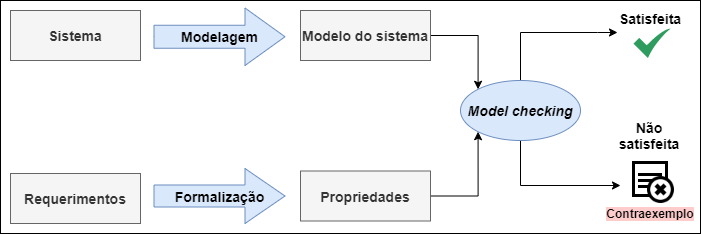
\includegraphics[scale=0.6]{figuras/model-checking.png}
 \fdireta{almakhour2020verification-survey}
\end{figure}

De forma geral, diversas linguagens formais e \textit{model checkers} podem ser utilizadas para modelagem e verificação de CIs. No trabalho de~\citeonline{nehai2018model-59}, um CI é modelado por meio da linguagem de entrada do \textit{model checker} NuSMV, o qual é utilizado para verificação de propriedades funcionais especificadas em CTL. Na estudo desenvolvido por~\citeonline{wang2020formal-04}, o código Solidity é traduzido para a linguagem formal MSVL, e o \textit{model checking} é aplicado para detecção da vulnerabilidade de reentrância. Também há exemplos de uso de Redes de Petri~\cite{liu2019formal-42} para modelagem, e de outros \textit{model checkers} como SPIN~\cite{bai2018formal-41, osterland2020model-58} e Spacer~\cite{marescotti2020accurate-10}.  

Um dos maiores desafios enfrentados no desenvolvimento de algoritmos de \textit{model checking} é a explosão de estados, que ocorre quando o modelo obtido a partir do código fornecido permite a exploração de uma quantidade excessivamente grande de estados, o que pode inviabilizar a aplicação desta técnica. Em razão disso, foram criados métodos alternativos de \textit{model checking} para tentar evitar a construção completa do grafo de estados, como o \textit{model checking} simbólico e o \textit{model checking} limitado~\cite{peled2019formal-methods}. Há também uma variação denominada \textit{model checking} estatístico, utilizada no trabalho de~\citeonline{abdellatif2018formal-44}, no qual o mecanismo de verificação calcula a probabilidade de sucesso em cada um dos cenários de ataque especificados. 

%No \textit{model checking} simbólico, conjuntos de estados são descritos de forma compacta por meio da representação simbólica dos estados obtida a partir de \sigla{DDB}{diagramas de decisão binário}, o que evita a exploração de caminhos de pesquisa redundantes~\cite{marescotti2018computing-17, shishkin2019debugging-22}.    

\subsubsection*{\textbf{Demonstração de teoremas}}

Na demonstração de teoremas, a modelagem do sistema e a especificação das propriedades é feita por meio de formalismos matemáticos~\cite{almakhour2020verification-survey}. Este método formal é utilizado para providenciar provas a partir de alguma lógica simbólica utilizando inferência dedutiva. Cada passo da demonstração introduz um axioma ou uma premissa e fornece uma afirmação, a qual consiste em uma consequência natural dos resultados previamente estabelecidos utilizando regras de inferência~\cite{singh2020survey-vulnerabilities-elsevier}. Os formalismos comumente utilizados para modelagem e especificação de propriedades são: lógica proposicional; lógica temporal (LTL, CTL); lógica de ordem superior e lógica de primeira ordem~\cite{harrison2008theorem, sun2020formal-03, yang2019fether-38, li2019formal-43}. 

\subsubsection*{\textbf{Verificação dedutiva}}

A verificação dedutiva consiste em gerar um conjunto de provas matemáticas a partir do sistemas e suas especificações. Se essas provas matemáticas se mostrarem verdadeiras, então isso implica na conformidade do sistema com sua especificação. Essa abordagem geralmente exige que seja fornecida uma sequência de teoremas que representam propriedades do sistema modelado e outras especificações como invariantes, pré-condições e pós-condições relacionadas com estas propriedades. O processo de verificação pode exigir trabalho manual, mas geralmente é executado com o auxílio de provadores de teoremas e SMT-solvers~\cite{ahrendt2016deductive-keybook, park2018formal-05, beillahi2020behavioral-15}. 

%- interpretação abstrata e refinamento de abstração

\subsection{\textit{Fuzzing}} \label{tex:fund:fuzzing}

Teste \textit{Fuzz}, ou \textit{fuzzing} é uma técnica para teste de software em que são fornecidos dados de entrada aleatórios chamados de \textit{FUZZ}~\cite{almakhour2020verification-survey}. Uma ferramenta de teste \textit{fuzz}, referida também como \textit{fuzzer}, gera entradas de teste para um programa alvo de forma iterativa e aleatória~\cite{klees2018fuzz-evaluating}.

Os \textit{fuzzers} geralmente seguem o seguinte procedimento~\cite{klees2018fuzz-evaluating}: (i) O processo é iniciado com a seleção de um conjunto de sementes de entrada com as quais o programa é testado; (ii) o \textit{fuzzer} cria repetitivamente mutações dessas entradas e avalia o programa testado; (iii) se o resultado obtido for considerado satisfatório, então o \textit{fuzzer} mantém a mutação de entrada para uso futuro e armazena o que foi observado; (iv) o \textit{fuzzer} é encerrado em duas situações, quando um determinado objetivo é alcançado (e.g., um determinado erro é encontrado, ou quando uma entrada causa o travamento do programa testado), ou quando o limite de tempo é atingido.

\subsection{Inteligência artificial} \label{tex:fund:ia}

Recentemente, técnicas de IA têm sido utilizadas para verificação e detecção de vulnerabilidades em CIs, principalmente as técnicas de \textit{machine learning}~\cite{xing2020new-08, sun2021attention-14, wang2020contractward-20} e \textit{deep learning}~\cite{gao2020checking-16, qian2020towards-96}. De forma geral, os métodos baseados em IA consistem na transformação de CIs com vulnerabilidades conhecidas para obtenção de vetores ou matrizes que representam padrões encontrados no código ou que indicam a presença de vulnerabilidades. Esses modelos de contratos vulneráveis são utilizados para treinar algoritmos de detecção, que verificam em outros contratos a presença de padrões similares aos encontrados nos contratos vulneráveis, indicando, assim, a presença de erros e vulnerabilidades. Na detecção de vulnerabilidades, são utilizadas técnicas como redes neurais, redes neurais convolucionais, floresta aleatória, redes de propagação de mensagens temporais, entre outras~\cite{xing2020new-08, zhuangsmart-84, sun2021attention-14, gao2020checking-16}. Em alguns casos, os modelos de contratos vulneráveis são adquiridos por meio da utilização de ferramentas baseadas em análise estática e execução simbólica, que são empregadas para rotulação das vulnerabilidades encontradas em cada contrato~\cite{wang2020contractward-20, momeni2019machine-54}.

%\cite{xing2020new-08} Recebe Bytecode - Que posteriormente é decompilado opcodes, que são segmentados, extraídos e combinados em uma matrix fatiada (slice matrix). Modelos de contratos vulnerávies para treinar algoritmos de machine learning. (auxílio da biblioteca tensorflow) Foi proposto o uso de fatiamento de matriz (slicing matrix) como elemento de reconhecimento de contratos vulneráveis. Três técnicas diferentes foram utilizados, baseadas em: Redes neurais, redes neurais convolucionais, e floresta aleatória; Endereço curto (shot address); Contrato guloso (greedy contract); integer overflow e underflow. \cite{sun2021attention-14} Bytecode -> opcode. Convolutional Learning Network(CNN). Reentrância, Integer overflow e underflow, Dependência de timestamp. \cite{wang2020contractward-20} Bigramas extraídos dos opcodes obtidos dos contratos. Rotulação dos rótulos feitos pela Oyente. \cite{momeni2019machine-54} Uso da Mythril e Slither para treinamento dos modelos. Contratos para treinamento são representados em vetores binários, onde cada byte representa a presença ou não de uma vulnerabilidade. \cite{zhuangsmart-84} superou a acurácia da SmartCheck, Oyente e Securify. dependência de timestamp e reentrância. Técnicas de ML graph neural networks (GNNs), degree-free graph convolutional neural network (DR-GCN), temporal message propagation network (TMP) \cite{gao2020checking-16} Ferramenta SmartEmbed. Deep learning (análise de similaridade). O código em Solidity é análisado e codificado em vetores numéricos que registram características léxicas, sintáticas e semânticas. Essa codificação do código é feita por meio de um parser que gera árvore sintática do código (Abstract Syntax Tree (AST)). Contratos vulneráveis conhecidos para treinamento. Serve para detecção de clones de código e também de erros. \cite{qian2020towards-96} Deep learning.

\subsection{Verificação em tempo de execução} \label{tex:fund:tempo-de-exec}

Métodos para verificação em tempo de execução consistem em instrumentalizar o código Solidity para que este tenha um sistema de monitoramento embutido. Desta forma, é possível monitorar os caminhos de execução e reagir à atividades suspeitas que podem levar à violação de propriedades predefinidas~\cite{wang2019contractguard-19, azzopardi2018monitoring-61, li2020securing-77}. Na ferramenta ContracLarva~\cite{azzopardi2018monitoring-61}, as partes envolvidas no projeto do contrato depositam uma quantia em Ether que fica bloqueada até o término da execução do contrato, e, em caso de detecção de violações de alguma propriedade, as partes prejudicadas são indenizadas, enquanto que aquelas que violaram alguma propriedade não recuperam o valor depositado. No estudo de~\citeonline{wang2019contractguard-19}, a ferramenta ContractGuard instrumentaliza o código fonte com um sistema de intrusão baseado em anomalia. Entretanto, a inserção de um mecanismo de monitoramento nos contratos tem como consequência o aumento do custo de execução, isto é, o gasto excessivo de \textit{gas}, o que representa a maior limitação encontrada em tais abordagens.~\cite{wang2019contractguard-19, azzopardi2018monitoring-61}.

\subsection{Lógica temporal} \label{tex:fund:logicas-temporais}

A lógica temporal é um formalismo usado para descrever sequências de transações entre estados em sistemas reativos~\cite{clarke2018model}. Portanto, uma fórmula lógica temporal geralmente é avaliada sobre um sistema de transição que modela uma especificação de um sistema~\cite{clarke2018model}. Na lógica temporal, o modelo é dado pela tupla $\mathcal{M} = (S, \rightarrow, L)$, em que $S$ é o conjunto de estados, $\rightarrow$ (ou $R$) $ \in S \times S$ é a relação de transição e $L \colon S \rightarrow 2^{AP}$ denota a função de rotulação dos estados com as proposições atômicas $AP$ verdadeiras no estado em que se encontram. Um exemplo de sistema de transição é apresentado na Figura~\ref{fig:temporal_grafo}, definido por:
\begin{itemize}
	\item $AP = \{p,q,r\}$
	\item $S = \{s_{0}, s_{1}, s_{2}\}$
	\item $\rightarrow = \{(s_{0}, s_{1}), (s_{1}, s_{0}), (s_{0}, s_{2}), (s_{1}, s_{2}), (s_{2}, s_{2})\}$
	\item $L(s_{0}) = \{p,q\}, L(s_{1}) = \{q, r\}, L(s_{2}) = \{r\}$
\end{itemize}

\begin{figure}[ht]
\caption{Exemplo de um sistema de transição.}
\label{fig:temporal_grafo}
\centering
\begin{tikzpicture}[>={Stealth[width=6pt,length=9pt]}, accepting/.style={double distance = 2pt, outer sep = 1pt + \pgflinewidth}, shorten >=1pt, auto]
\draw (158.0pt, -70.0pt)node[state, label=right:$s_{0}$](0){$p,q$};
\draw (80.0pt, -171.0pt)node[state, label=below:$s_{1}$](1){$q,r$};
\draw (220.0pt, -171.0pt)node[state, label=right:$s_{2}$](2){$r$};
\path[->] (2) edge[loop below] node{}(2);
\path[->] (1) edge node{}(2);
\path[->] (0) edge node{}(2);
\path[->] (1) edge[bend left] node{}(0);
\path[->] (0) edge[bend left] node{}(1);
\end{tikzpicture}
\fdireta{huth2004logic}
\end{figure}

Uma fórmula lógica temporal pode ser verdadeira ou falsa dependendo do modelo no qual é interpretada. O conjunto de estados representam a evolução do sistema ao longo do tempo e as fórmulas são avaliadas em cada estado do sistema. Portanto, a noção estática de verdade é substituída pela noção dinâmica de evolução dos estados do sistema ao longo do tempo~\cite{clarke2018model}. A lógica temporal pode ser dos tipos linear ou ramificada, as quais são discutidas a seguir.

\subsubsection*{\textbf{Lógica temporal linear}}

Na lógica linear (do ingês, \sigla{LTL}{\textit{linear tree logic}}), o tempo é tratado como se cada momento tivesse apenas um único futuro possível, logo, as fórmulas são interpretadas como sequências lineares, ou caminhos. A LTL possui conectivos que se referem ao futuro, e suas fórmulas são interpretadas sobre uma sequência de estados (i.e., o caminho). Um caminho é uma sequência finita não vazia denotada por $\pi = \langle \pi_{0}, \pi_{1}, \ldots, \pi_{n-1} \rangle$, em que os estados $\pi_{0}, \pi_{1}, \ldots, \pi_{n-1} \in S$ e $(\pi_{i}, \pi_{i-1}) \in R$ para todo $0 \leq i < n-1$. O tamanho de um caminho é denotado por $|\pi|=\infty$. Um caminho infinito é denotado por $\pi = \langle \pi_{0}, \pi_{1}, \pi_{3}, \ldots \rangle$ com tamanho $|\pi| = \infty$. Todo caminho que não pode ser estendido é considerado maximal, logo, qualquer caminho infinito é maximal~\cite{muller1999invited}. A sintaxe de uma fórmula LTL é composta de proposições atômicas e gerada conforme segue:
\begin{equation}
\varphi ::= \top~|~\bot~|~p~|~\neg \varphi~|~\varphi \vee \varphi~|~\varphi \rightarrow \varphi~|~X\varphi~|~F\varphi~|~G\varphi~|~\varphi U \varphi'
\end{equation}

Assim como na lógica proposicional, os valores lógicos avaliados como verdadeiro e falso são representados pelos símbolos $\top$ e $\bot$, respectivamente, além dos operadores lógicos $\neg$, $\wedge$, $\vee$ e $\rightarrow$, que também têm o mesmo significado. Já o símbolo $p$ representa um identificador das proposições, e os operadores $X$, $F$, $G$ e $U$, são usados para especificar situações temporais de uma fórmula. A expressão $X\varphi$ (após $\varphi$) indica que a proposição $\varphi$ é verdadeira no próximo estado. Já a expressão $F\varphi$ (afinal, $\varphi$) configura que em algum estado futuro da computação, $\varphi$ é verdadeira, enquanto que $G\varphi$ (sempre $\varphi$) indica que $\varphi$ é verdadeira em todos os estados do caminho de computação. Enfim, a expressão $\varphi U \varphi'$ ($\varphi$ até que $\varphi'$) significa que a proposição $\varphi$ deve ser verdadeira em todos os estados até que $\varphi$ seja verdadeira~\cite{mura2016, muller1999invited}. 

Uma fórmula $\alpha$ em LTL é satisfeita se existe um modelo $\mathcal{M}$ e um caminho $\pi$ tal que $\mathcal{M}, \pi \models \varphi$, ou seja, um modelo no qual o caminho $\pi$ satisfaz a fórmula $\varphi$. Um caminho é formado por uma sequência de estados $s$ e suas posições são indexadas partindo de $\pi_{1}$ até $\pi_{n}$, em que $n$ determina a quantidade de posições de $\pi$. Sendo $\pi$ um dado caminho de $\mathcal{M}$, as relações de satisfação $\models$ e $\nvDash$ indicam se uma fórmula LTL é satisfeita ou não, respectivamente, por $\pi$, como exposto na Figura~\ref{fig:ltl_sem}. 

\begin{figure}[ht]
	\caption{Semântica da LTL.} \label{fig:ltl_sem}
	\centering
	\begin{align}
	&\pi \models \top \label{eq:l1} \\
	&\pi \nvDash \bot \label{eq:l2} \\
	&\pi \models p \Longleftrightarrow p \in L(\pi_{1}) \label{eq:l3} \\
	&\pi \models \neg \varphi \iff \pi \not \models \varphi \label{eq:l4} \\
	&\pi \models \varphi \wedge \varphi' \iff \pi \models \varphi \mbox{ e } \pi \models \varphi' \label{eq:l5}\\
	&\pi \models \varphi \vee \varphi' \iff \pi \models \varphi \mbox{ ou } \pi \models \varphi' \label{eq:l6}\\
	&\pi \models \varphi \to \varphi' \iff \pi \models \varphi \mbox{ sempre que } \pi \models \varphi' \label{eq:l7}\\
	&\pi \models X\varphi \iff \pi_2 \models \varphi \label{eq:l8}\\
	&\pi \models G\varphi \iff \forall i \geq 1 \mid \pi_i \models \varphi \label{eq:l9}\\
	&\pi \models F\varphi \iff \exists i \geq 1 \mid \pi_i \models \varphi \label{eq:l10}\\
	&\pi \models \varphi U \varphi' \iff \exists i \geq 1 \mid \pi_i \models \varphi' \mbox{ e } \forall j = 1 \wedge j < i \mid \pi_j \models \varphi \label{eq:l11}
	\end{align}
	\fdireta{huth2004logic}
\end{figure}

Nas definições~\ref{eq:l1} e~\ref{eq:l2} da Figura~\ref{fig:ltl_sem} são indicadas as proposições verdadeiras e falsas, respectivamente. Na definição~\ref{eq:l3} é dito que a proposição $p$ só é válida se estiver no primeiro estado do caminho. Nas proposições~\ref{eq:l4} à~\ref{eq:l7} são definidos os conectivos proposicionais da lógica proposicional. Em~\ref{eq:l8}, o operador $X$ denota que a fórmula $\varphi$ é satisfeita no próximo estado, no caso, a segunda posição do caminho. As definições~\ref{eq:l9} e~\ref{eq:l10} representam os operadores $G$ e $F$ que apontam, respectivamente, que a fórmula $\varphi$ é verdadeira em todas ou em pelo menos uma posição de $\pi$. Por fim, a definição~\ref{eq:l11} representa o operador $U$, expressando que, para toda posição antecessora à $\pi_{i}$, a fórmula $\varphi$ é verdadeira, caso contrário, a proposição $\varphi'$ é verdadeira.

Diversas propriedades podem ser verificadas com fórmulas LTL, tais como as de segurança, de vivacidade, e de progresso~\cite{huth2004logic, mura2016}. ~\citeonline{huth2004logic} descrevem algumas propriedades que podem ser representadas em sistemas reais, considerando um sistema especificado com as proposições $ocupado$, $requisitado$, $iniciado$, $pronto$ e $habilitado$, como nos exemplos a seguir:

\begin{itemize}
	\item O sistema não pode ter $iniciado$ e ainda não estar $pronto$ para atender requisições: 
	\begin{equation}
	G\neg(iniciado\wedge\neg\;pronto)
	\end{equation} 
	\item Em todo sistema, se é $requisitado$ algum recurso, o requisitante deve ser $respondido$:
	\begin{equation}
	G(requisitado \to F\;respondido)
	\end{equation}
	\item Um processo é $habilitado$ infinitas vezes em todo o caminho de computação: 
	\begin{equation}
	GF\;habilitado 
	\end{equation}
	\item Um elevador subindo para o segundo andar não muda sua direção quando houver passageiros que desejam ir para o quinto andar: 
	\begin{equation}
	G(andar2 \wedge subindo \wedge pressionadoBotao5 \to (subindo U andar5))
	\end{equation}
\end{itemize}

\subsubsection*{\textbf{Lógica temporal ramificada}}

A lógica temporal ramificada (do inglês, \sigla{CTL}{\textit{computational tree logic}}), ou lógica de computação em árvore (CTL), é capaz de representar sistemas de transições de estados em que o futuro não é determinado, ou seja, quando há uma variedade de possíveis caminhos que podem ser tomados a partir de um determinado estado. Sendo assim, a evolução do sistema ao longo do tempo pode ser representada por uma árvore que retrata todas as execuções possíveis~\cite{huth2004logic}. Na Figura~\ref{fig:ctl_ex}, à esquerda, é apresentado um modelo de estados, e à direita, a árvore de computação que representa as mudanças de estados, retratados pelo rótulo do nó e o nível de profundidade da execução.

\begin{figure}[ht]
    \caption{Exemplo de árvore de computação num sistema de transição.} \label{fig:ctl_ex}
	\centering
	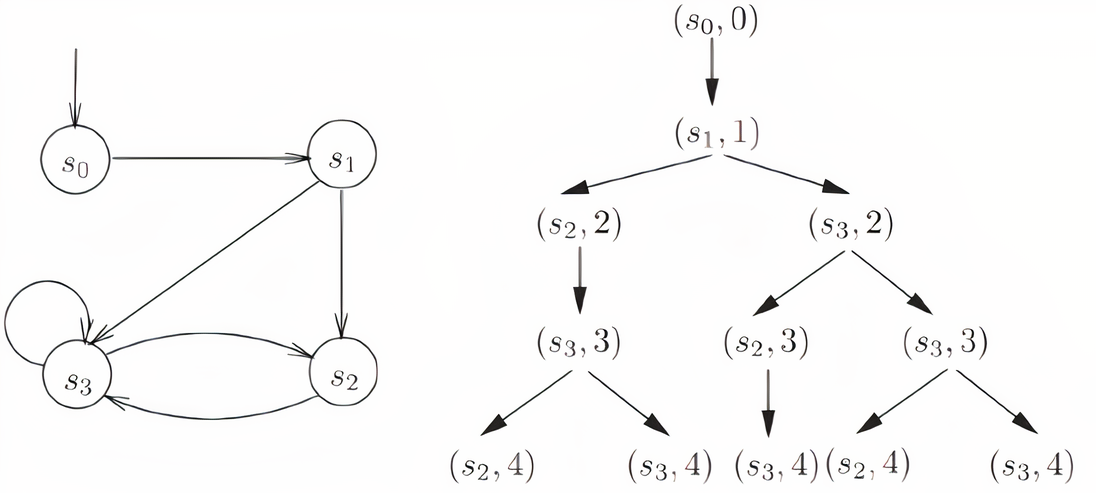
\includegraphics[width=0.8\textwidth]{figuras/ctl_ex.png}
	\fdireta{huth2004logic}
\end{figure}

A sintaxe de construção de fórmulas CTL estende a LTL e adiciona os operadores existencial ($E$) e universal ($A$), e consiste em:
\begin{align}
& \varphi ::= \top \mid \perp \mid p \mid \neg \varphi \mid \varphi \wedge \varphi \mid \varphi\vee\varphi \mid \varphi \to \varphi \mid \nonumber \\ 
& AX\varphi \mid EX\varphi \mid AF\varphi \mid EF\varphi \mid AG\varphi \mid EG\varphi \mid A[\varphi U \varphi]\mid E[\varphi U \varphi] \label{eq:ctl}
\end{align}

Como exposto na definição~\ref{eq:ctl}, os conectivos temporais da CTL são usados em pares, sendo o primeiro um quantificador, denotado por $A$ ou $E$, enquanto que o segundo é um operador temporal, usado da mesma forma que na LTL. O quantificador $A$ expressa que, a partir de um determinado estado, a propriedade é verdadeira para todos os caminhos de computação possíveis. O operador $E$ sugere que, a partir de um determinado estado, há ao menos um caminho em que a propriedade é verdadeira~\cite{katoen1999concepts}. Alguns exemplos de fórmulas CTL são apresentados a seguir: 
\begin{itemize}
	\item É possível chegar a um estado em que o sistema está $iniciado$ mas não está $pronto$? 
	\begin{equation}
	EF(iniciado \wedge \neg pronto)
	\end{equation}
	\item Em qualquer caminho e em todo este caminho, se algum recurso é $requisitado$, ele eventualmente é $reconhecido$? 
	\begin{equation}
	AG(requisitado \to AF\;reconhecido)
	\end{equation}
	\item Um determinado processo está $habilitado$ infinitamente em cada caminho de computação. 
	\begin{equation}
	AG(AF\;habilitado)
	\end{equation}
\end{itemize}

Assim como na LTL, as fórmulas em CTL são interpretadas sobre os caminhos a partir de estados em um sistema de transição~\cite{katoen1999concepts}. Dado o modelo de transição $\mathcal{M} = (S, \rightarrow, L)$, a relação de satisfação $\mathcal{M}, s \models \varphi$ pode ser dada indutivamente conforme é exibido na Figura~\ref{fig:ctl_sem}, em que $s \in \mathcal{M}$ e $\varphi$ é uma fórmula em CTL~\cite{mura2016}.

Na CTL, os quantificadores existencial e universal podem ser aninhados para expressar propriedades mais complexas. Por exemplo, uma propriedade em que para todo caminho de computação sempre é possível retornar para o estado inicial, pode ser representada por $AG~(EF~(inicio))$. A partir desta fórmula CTL, interpreta-se que, em todo estado do sistema ($G$), para todo caminho de computação ($A$), existe a possibilidade ($E$) de eventualmente retornar ao início ($F~inicio$)~\cite{baier2008principles}.

\begin{figure}[H]
    \caption{Semântica da CTL.} \label{fig:ctl_sem}
	\centering
	\begin{align}
	&\mathcal{M},s  \models  \top \\
	&\mathcal{M},s  \not\models  \perp \\
	&\mathcal{M},s  \models  p \iff p \in L(s) \\
	&\mathcal{M},s  \models  \neg \varphi \iff \pi \not \models \varphi \\
	&\mathcal{M},s  \models  \varphi \wedge \varphi' \iff \mathcal{M},s \models \varphi \mbox{ e } \mathcal{M},s \models \varphi' \\
	&\mathcal{M},s  \models  \varphi \vee \varphi' \iff \mathcal{M},s \models \varphi \mbox{ ou } \mathcal{M},s \models \varphi' \\
	&\mathcal{M},s  \models  \varphi \to \varphi' \iff \mathcal{M},s \not\models \varphi \mbox{ ou } \mathcal{M},s \models \varphi' \\
	&\mathcal{M},s  \models  AX\varphi \iff \forall s_1 \mid s\to s_1 \mbox{ com } \mathcal{M}, s_1 \models \varphi \\
	&\mathcal{M},s  \models  EX\varphi \iff \exists s_1 \mid s\to s_1 \mbox{ com } \mathcal{M}, s_1 \models \varphi \\
	&\mathcal{M},s  \models  AG\varphi \iff \forall \pi = s_1\to s_2\to s_3\to \dots \mid s_1 = s \mbox{ e } \forall s_i \in \pi \mbox{ com } \mathcal{M}, s_i \models \varphi \\
	&\mathcal{M},s  \models  EG\varphi \iff \exists \pi = s_1\to s_2\to s_3\to \dots \mid s_1 = s \mbox{ e } \forall s_i \in \pi \mbox{ com } \mathcal{M}, s_i \models \varphi \\
	&\mathcal{M},s  \models  AF\varphi \iff \forall \pi = s_1\to s_2\to s_3\to \dots \mid s_1 = s \mbox{ e } \exists s_i \in \pi \mid \mathcal{M}, s_i \models \varphi \\
	&\mathcal{M},s  \models  EF\varphi \iff \exists \pi = s_1\to s_2\to s_3\to \dots \mid s_1 = s \mbox{ e } \exists s_i \in \pi \mid \mathcal{M}, s_i \models \varphi \\
	&\mathcal{M},s  \models  A[\varphi U \varphi'] \iff \forall \pi = s_1\to s_2\to s_3\to \dots \mid s_1 = s \exists s_i \in \pi \mid \\
	&\mathcal{M}, s_i \models \varphi' \mbox{ e } \forall j < i \mbox{ com }  \mathcal{M}, s_j \models \varphi \\
	&\mathcal{M},s  \models  E[\varphi U \varphi'] \iff \exists \pi = s_1\to s_2\to s_3\to \dots \mid s_1 = s \exists s_i \in \pi \mid \\
	&\mathcal{M}, s_i \models \varphi' \mbox{ e } \forall j < i \mbox{ com }  \mathcal{M}, s_j \models \varphi
	\end{align}
	\fdireta{mura2016}	
\end{figure}

%#falar do correct-by-construction, que é proativo

%A interpretação abstrata formaliza a ideia de abstração de estruturas matemáticas que visam obter solidez na análise de programas por meio do fornecimento de uma semântica aproximada de um programa~\cite{cousot2012formal}. A semântica concreta é uma caracterização matemática que formaliza o conjunto de todas as execuções possíveis em todos os ambientes de execução possíveis. No contexto dos CIs, interpretação abstrata ignora certas instruções enquanto executa o bytecode por meio de tradução de instruções para algum outro formalismo, e então explora todas as execuções possíveis~\cite{almakhour2020verification-survey}.

% Análise de contaminação está englobada em análise dinâmica?